\subsection{Verification}
\label{sec:appendix_verification}
In this section we verify the SSTE algorithm on canonical autonomous test cases and on an analytical non-autonomous problem, and we measure every case through the growth functional \(g(T)\) of \eqref{eq:appendix_growth_functional}. We define the relative error as
\begin{equation}
  \varepsilon_{\mathrm{rel}}(T)
  =
  \frac{
    \left|\widehat{g}(T)-g_{\mathrm{ref}}(T)\right|
  }{
    \left|g_{\mathrm{ref}}(T)\right|
  },
  \label{eq:verification_relative_error}
\end{equation}
where \(g_{\mathrm{ref}}\) is the reference value and \(\widehat{g}\) is the corresponding SSTE estimate. The reference is exact in every case considered, but its origin differs. For autonomous problems the linearized operators are constant in time, so the procedure is unchanged except that the propagator can be formed and stored explicitly; the reference is then the trace evaluated from the exponential propagator. For the fully non-autonomous case we derive a closed-form solution, and the reference is the resulting analytical expression.

The verification cases are organized as follows. \Cref{sec:appendix_verification_gl} uses an autonomous complex Ginzburg--Landau problem, so the exact matrix-exponential reference is available and the estimator can be tested without ambiguity from time-dependent coefficients. This case also provides the direct comparison between SSTE and the naive \(\mathsfbi{C}_{00}^{z}\) truncation discussed in \Cref{sec:appendix_necessity_sste}. \Cref{sec:appendix_verification_poiseuille} repeats both the autonomous matrix-exponential verification and the convergence-cost comparison for plane Poiseuille flow, providing a fluid-dynamical test of the same trace construction. \Cref{sec:appendix_verification_nonautonomous} uses a fully non-autonomous scalar problem with a closed-form trace reference, isolating the effect of time-dependent coefficients.

\subsubsection{Complex Ginzburg--Landau}
\label{sec:appendix_verification_gl}
\begin{figure}
    \centering
    \begin{minipage}[t]{0.48\textwidth}
        \centering
        \vspace{0pt}
        % This file was created by matlab2tikz.
%
\definecolor{mycolor1}{rgb}{0.20000,0.40000,0.60000}%
%
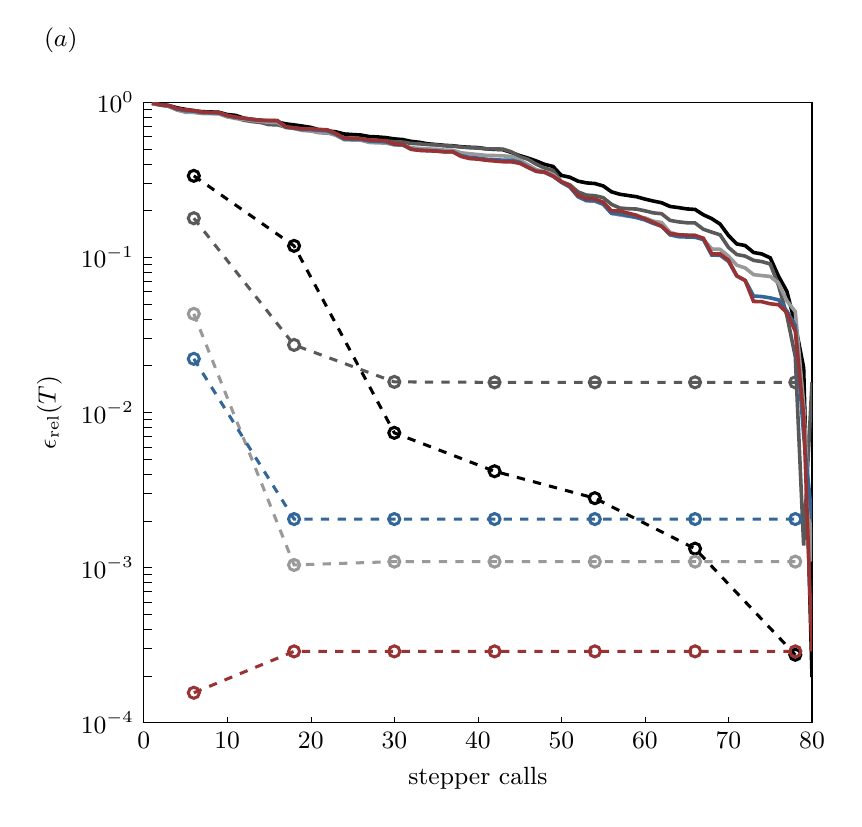
\begin{tikzpicture}

\begin{axis}[%
width=11.252in,
height=7.131in,
at={(1.887in,0.962in)},
scale only axis,
clip=true,
separate axis lines,
every outer x axis line/.append style={black},
every x tick label/.append style={font=\color{black}},
every x tick/.append style={black},
xmin=0,
xmax=80,
xlabel={stepper calls},
every outer y axis line/.append style={black},
every y tick label/.append style={font=\color{black}},
every y tick/.append style={black},
ymode=log,
ymin=0.0001,
ymax=1,
yminorticks=true,
ylabel={$\epsilon_{\mathrm{rel}}(T)$},
axis background/.style={fill=white},
clip=true,
clip mode=individual,
axis lines=box,
xtick pos=bottom,
ytick pos=left,
tick align=inside,
major tick length=2pt,
width=0.7\linewidth,
height=0.65\linewidth,
every axis/.append style={font=\fontsize{9}{9}\selectfont},xlabel style={font=\fontsize{9}{9}\selectfont},title style={font=\fontsize{9}{9}\selectfont},
legend style={font=\fontsize{8}{9}\selectfont,inner sep=1pt,row sep=1pt,column sep=2pt,nodes={scale=1.00},draw=none},legend image post style={xscale=0.35},
legend columns=1,
scaled x ticks=false,
tick label style={/pgf/number format/fixed,/pgf/number format/precision=2},
every x tick label/.append style={font=\fontsize{9}{9}\selectfont\color{black}},
every y tick label/.append style={font=\fontsize{9}{9}\selectfont\color{black}},
,,
colormap={sigmamap}{rgb(0.0000)=(0.0200,0.1880,0.3800); rgb(0.1000)=(0.0743,0.3456,0.5616); rgb(0.2000)=(0.1918,0.4980,0.7060); rgb(0.3000)=(0.3890,0.6708,0.8226); rgb(0.4000)=(0.7552,0.8682,0.9228); rgb(0.5000)=(0.9690,0.9689,0.9689); rgb(0.6000)=(0.9425,0.8044,0.7614); rgb(0.7000)=(0.8767,0.4910,0.4020); rgb(0.8000)=(0.7869,0.2866,0.2470); rgb(0.9000)=(0.6186,0.1239,0.1568); rgb(1.0000)=(0.4040,0.0000,0.1220)}
]
\addplot [color=black, line width=1.3pt, forget plot]
  table[row sep=crcr]{%
1	0.985165464502917\\
2	0.971048359830997\\
3	0.951205179050231\\
4	0.919681047700775\\
5	0.899249412820878\\
6	0.880805994430103\\
7	0.868459742494046\\
8	0.865199492680536\\
9	0.861114197062287\\
10	0.832525113113597\\
11	0.822398689108786\\
12	0.788670148690936\\
13	0.775021625627415\\
14	0.764549352578276\\
15	0.747746973613479\\
16	0.745712139733251\\
17	0.724965063859842\\
18	0.713974519830427\\
19	0.701444244155202\\
20	0.688482774619424\\
21	0.663182110301451\\
22	0.65435357265626\\
23	0.64407505382054\\
24	0.624129625964055\\
25	0.618414678614345\\
26	0.614229876610716\\
27	0.600565092768903\\
28	0.597031889384245\\
29	0.591240547176463\\
30	0.579989136718529\\
31	0.574332747631998\\
32	0.558906071472685\\
33	0.551424866729417\\
34	0.539182540890269\\
35	0.533524060767838\\
36	0.52717094141623\\
37	0.523571656178599\\
38	0.516042372207813\\
39	0.512332268723539\\
40	0.509670785497178\\
41	0.500782949538627\\
42	0.496546792309842\\
43	0.494342949858862\\
44	0.474330601756383\\
45	0.45263687517021\\
46	0.436463402022355\\
47	0.41765607247181\\
48	0.397465607198713\\
49	0.385282284592009\\
50	0.337283356987566\\
51	0.328513798162926\\
52	0.309670329668666\\
53	0.301926775381416\\
54	0.299026111763803\\
55	0.288612391923131\\
56	0.264457019190453\\
57	0.254980536533236\\
58	0.250205782373461\\
59	0.245812576451499\\
60	0.237374855379344\\
61	0.230549355537883\\
62	0.224861889966195\\
63	0.212799059810108\\
64	0.209293996703853\\
65	0.205196913687323\\
66	0.203571124582919\\
67	0.188035812467885\\
68	0.177630310730338\\
69	0.16372654312346\\
70	0.138302991694355\\
71	0.122002256923464\\
72	0.119097970006177\\
73	0.107519625210511\\
74	0.105067727551673\\
75	0.0992037278314537\\
76	0.0754210347718126\\
77	0.0602465034532608\\
78	0.0366705573794107\\
79	0.019419822005287\\
80	0.000197351436241734\\
};
\addplot [color=black, dashed, line width=1.1pt, mark size=2.0pt, mark=o, mark options={solid, black}, forget plot]
  table[row sep=crcr]{%
6	0.335159987761167\\
18	0.118531569790602\\
30	0.00739365023044105\\
42	0.00417927746508909\\
54	0.00280275867247948\\
66	0.001325154662104\\
78	0.000274288373235347\\
};
\addplot [color=white!35!black, line width=1.3pt, forget plot]
  table[row sep=crcr]{%
1	0.978599504948092\\
2	0.958939501992847\\
3	0.939693066967005\\
4	0.89261026284617\\
5	0.867840917394025\\
6	0.861406077656702\\
7	0.852698239057536\\
8	0.85017245615521\\
9	0.847032144185355\\
10	0.80729432471463\\
11	0.793416282120727\\
12	0.765630153360495\\
13	0.74988185038214\\
14	0.740470036675323\\
15	0.716426184465566\\
16	0.715341748661657\\
17	0.691584384991789\\
18	0.683455781101978\\
19	0.670675562334103\\
20	0.654454550999417\\
21	0.637112149433065\\
22	0.633257778866529\\
23	0.620317618750451\\
24	0.588720020973351\\
25	0.585945706960771\\
26	0.582267838430227\\
27	0.56742924037083\\
28	0.565364720145365\\
29	0.562807616623031\\
30	0.555634500442104\\
31	0.553314809191816\\
32	0.54238243410962\\
33	0.539039247828093\\
34	0.532643096219939\\
35	0.530584870874834\\
36	0.522539364472817\\
37	0.521445234589325\\
38	0.513154688684804\\
39	0.508839959353012\\
40	0.505939514085901\\
41	0.500655814429845\\
42	0.499712265513766\\
43	0.498404391560835\\
44	0.478878943258887\\
45	0.445626597424573\\
46	0.428464859611121\\
47	0.398258275036155\\
48	0.376128564976229\\
49	0.362789243735769\\
50	0.307295386037411\\
51	0.293601467871381\\
52	0.263957921658544\\
53	0.251759619862065\\
54	0.249676687234887\\
55	0.242489853789401\\
56	0.219495168292962\\
57	0.207859611903422\\
58	0.205754176866974\\
59	0.204741582868334\\
60	0.199458164115086\\
61	0.193520310988052\\
62	0.190931637714247\\
63	0.173087985360088\\
64	0.169340146062514\\
65	0.167072941945809\\
66	0.166542467767846\\
67	0.151614680982998\\
68	0.145368741746296\\
69	0.139618579434393\\
70	0.115866788291259\\
71	0.104232963892324\\
72	0.101843105302551\\
73	0.0955708834689444\\
74	0.0938174024887371\\
75	0.0906079543094753\\
76	0.0657956360552881\\
77	0.0418853536153708\\
78	0.0228826914806503\\
79	0.00138771895001788\\
80	0.0156460030015282\\
};
\addplot [color=white!35!black, dashed, line width=1.1pt, mark size=2.0pt, mark=o, mark options={solid, white!35!black}, forget plot]
  table[row sep=crcr]{%
6	0.178634994647454\\
18	0.0272494655305371\\
30	0.0157452937165598\\
42	0.0156391308471297\\
54	0.0156432097817025\\
66	0.0156460997728516\\
78	0.0156460065903751\\
};
\addplot [color=white!60!black, line width=1.3pt, forget plot]
  table[row sep=crcr]{%
1	0.983939814725101\\
2	0.958621292050389\\
3	0.941410908329715\\
4	0.890755899497388\\
5	0.861457015736498\\
6	0.859985130675222\\
7	0.845697130140114\\
8	0.84384524991711\\
9	0.840712634135543\\
10	0.806066660950854\\
11	0.785220616474763\\
12	0.776763649448303\\
13	0.761103340890232\\
14	0.75261633371115\\
15	0.740564558251317\\
16	0.739651588083636\\
17	0.686174570596409\\
18	0.676538220042228\\
19	0.65747615287434\\
20	0.651761925296852\\
21	0.640299018596555\\
22	0.636199216480547\\
23	0.610879445340382\\
24	0.573000938865489\\
25	0.570269997442903\\
26	0.568735320710756\\
27	0.550363133482551\\
28	0.546783209951033\\
29	0.545147664528803\\
30	0.530625903954825\\
31	0.528389559501782\\
32	0.508318851954079\\
33	0.503980652374716\\
34	0.499613192675354\\
35	0.49763637312336\\
36	0.490959101835251\\
37	0.490643493508232\\
38	0.472132561173985\\
39	0.46529930178891\\
40	0.459836536188394\\
41	0.454070526874192\\
42	0.453084808068927\\
43	0.450921515878575\\
44	0.446915469987828\\
45	0.423482412433708\\
46	0.395423667568545\\
47	0.367204866683023\\
48	0.356292784685205\\
49	0.341663964243568\\
50	0.306891857435353\\
51	0.285139234618715\\
52	0.246301072832208\\
53	0.231967547990899\\
54	0.230547619059275\\
55	0.221083463022862\\
56	0.192621792750176\\
57	0.187439295663882\\
58	0.184303648641886\\
59	0.182138524821364\\
60	0.179570703186825\\
61	0.171154224360516\\
62	0.167433487565166\\
63	0.145003386402656\\
64	0.139611153942317\\
65	0.139222997248754\\
66	0.138620251364076\\
67	0.130288551990365\\
68	0.113200339183079\\
69	0.112642085997531\\
70	0.101776616986649\\
71	0.0890035156036651\\
72	0.0854020580954648\\
73	0.077391766903902\\
74	0.0762840444580965\\
75	0.0753165799713176\\
76	0.0680914430609462\\
77	0.0523770125267109\\
78	0.0446863165468323\\
79	0.0113900519737571\\
80	0.00109306870352377\\
};
\addplot [color=white!60!black, dashed, line width=1.1pt, mark size=2.0pt, mark=o, mark options={solid, white!60!black}, forget plot]
  table[row sep=crcr]{%
6	0.0432217565843151\\
18	0.00104058419757173\\
30	0.00109300796967562\\
42	0.00109306851668768\\
54	0.00109306870455549\\
66	0.00109306870351742\\
78	0.00109306870352434\\
};
\addplot [color=mycolor1, line width=1.3pt, forget plot]
  table[row sep=crcr]{%
1	0.989811891709964\\
2	0.960431859012181\\
3	0.947709764979468\\
4	0.902376300114507\\
5	0.881075920619318\\
6	0.876674455805922\\
7	0.856885350128844\\
8	0.855090827494591\\
9	0.851761640525362\\
10	0.819320189184422\\
11	0.797292548273364\\
12	0.78806122225905\\
13	0.77276006590294\\
14	0.764282501804924\\
15	0.76071644434043\\
16	0.759703269063204\\
17	0.691619520587041\\
18	0.67967319361489\\
19	0.666621616328036\\
20	0.665504318632122\\
21	0.658670748743334\\
22	0.653705159150912\\
23	0.621556267060521\\
24	0.579768859923312\\
25	0.576997067249284\\
26	0.575868845616789\\
27	0.562810814189649\\
28	0.55797512494194\\
29	0.555658984500403\\
30	0.533488707883595\\
31	0.530480999056352\\
32	0.498123892171704\\
33	0.491116268851211\\
34	0.487948530398078\\
35	0.485573568159683\\
36	0.479551659861754\\
37	0.479359417296565\\
38	0.452077992888222\\
39	0.440933079350967\\
40	0.436152475342342\\
41	0.428890724024518\\
42	0.426217957695805\\
43	0.42258233338666\\
44	0.422254731169116\\
45	0.409952512737682\\
46	0.381810352992008\\
47	0.358308180091778\\
48	0.352175878101747\\
49	0.333306977167566\\
50	0.30424016970697\\
51	0.284178935698881\\
52	0.245756387656101\\
53	0.232000781397229\\
54	0.231310588412865\\
55	0.220004381709227\\
56	0.191907614754701\\
57	0.190463142463489\\
58	0.184969423564124\\
59	0.180402954768267\\
60	0.174144315703504\\
61	0.165465646833326\\
62	0.158712453070042\\
63	0.139617470060995\\
64	0.135879800133814\\
65	0.135207205933744\\
66	0.134716855584887\\
67	0.130151348694189\\
68	0.103306056164728\\
69	0.103176492744065\\
70	0.0941986632569092\\
71	0.0758320657443923\\
72	0.0710547597258276\\
73	0.0563570401697191\\
74	0.0558645644393192\\
75	0.0547663759366945\\
76	0.0531627847504146\\
77	0.0449587446280415\\
78	0.036338931906693\\
79	0.00714351915577783\\
80	0.002055929390514\\
};
\addplot [color=mycolor1, dashed, line width=1.1pt, mark size=2.0pt, mark=o, mark options={solid, mycolor1}, forget plot]
  table[row sep=crcr]{%
6	0.0221710184949555\\
18	0.00205572676526485\\
30	0.00205592952111303\\
42	0.00205592939052286\\
54	0.0020559293905168\\
66	0.00205592939051692\\
78	0.0020559293905112\\
};
\addplot [color=red!60!teal, line width=1.3pt, forget plot]
  table[row sep=crcr]{%
1	0.992325618839863\\
2	0.961016066817814\\
3	0.951208342921825\\
4	0.909270854860793\\
5	0.89254895682782\\
6	0.884815513639991\\
7	0.862290154659604\\
8	0.860415877005582\\
9	0.857853229850865\\
10	0.822332385875221\\
11	0.801433628859122\\
12	0.787904543949321\\
13	0.774317514752259\\
14	0.765141215814968\\
15	0.762530829118749\\
16	0.761325433853939\\
17	0.694682953325543\\
18	0.682341731535508\\
19	0.674346656399483\\
20	0.672786566648059\\
21	0.668200119625061\\
22	0.663293053353033\\
23	0.629081819149951\\
24	0.586888228823027\\
25	0.584317228262044\\
26	0.581314029745595\\
27	0.571490377868498\\
28	0.566770176814566\\
29	0.563935424311444\\
30	0.537455260735946\\
31	0.53422339882455\\
32	0.497334856023746\\
33	0.488809171678629\\
34	0.486072051456463\\
35	0.483504725005103\\
36	0.478304543183782\\
37	0.478240020525966\\
38	0.446736796169955\\
39	0.433120419580013\\
40	0.429548615138443\\
41	0.422298926512988\\
42	0.417698915367519\\
43	0.413275061006734\\
44	0.412531808256351\\
45	0.40388650613073\\
46	0.379494267012634\\
47	0.358844828047536\\
48	0.354638192262945\\
49	0.333453830121188\\
50	0.307032096596556\\
51	0.289435507933016\\
52	0.251135032099835\\
53	0.238193191630314\\
54	0.237783085631403\\
55	0.226677193556239\\
56	0.199360448424778\\
57	0.198959877325978\\
58	0.192612715272565\\
59	0.186689944541466\\
60	0.177117654749482\\
61	0.168016765002079\\
62	0.158442443672403\\
63	0.142320577140866\\
64	0.140036078567272\\
65	0.138761648579695\\
66	0.138314633879418\\
67	0.132805255890634\\
68	0.105232681267841\\
69	0.105081998102503\\
70	0.0959096699196229\\
71	0.0759144093102118\\
72	0.070894907510888\\
73	0.0519731430204992\\
74	0.0517514147346468\\
75	0.0501827934196301\\
76	0.049479744716153\\
77	0.0439304260189536\\
78	0.0333957003281456\\
79	0.00955117552443943\\
80	0.000288500251500087\\
};
\addplot [color=red!60!teal, dashed, line width=1.1pt, mark size=2.0pt, mark=o, mark options={solid, red!60!teal}, forget plot]
  table[row sep=crcr]{%
6	0.000156112389094138\\
18	0.000288490466867784\\
30	0.000288500251553511\\
42	0.00028850025150066\\
54	0.000288500251500851\\
66	0.000288500251497798\\
78	0.000288500251498943\\
};
\node[right, align=left, inner sep=0]
at (rel axis cs:-0.15,1.1) {$(a)$};
\end{axis}
\end{tikzpicture}%
    \end{minipage}
    \hfill
    \begin{minipage}[t]{0.48\textwidth}
        \centering
        \vspace{0pt}
        % This file was created by matlab2tikz.
%
\definecolor{mycolor1}{rgb}{0.20000,0.40000,0.60000}%
%
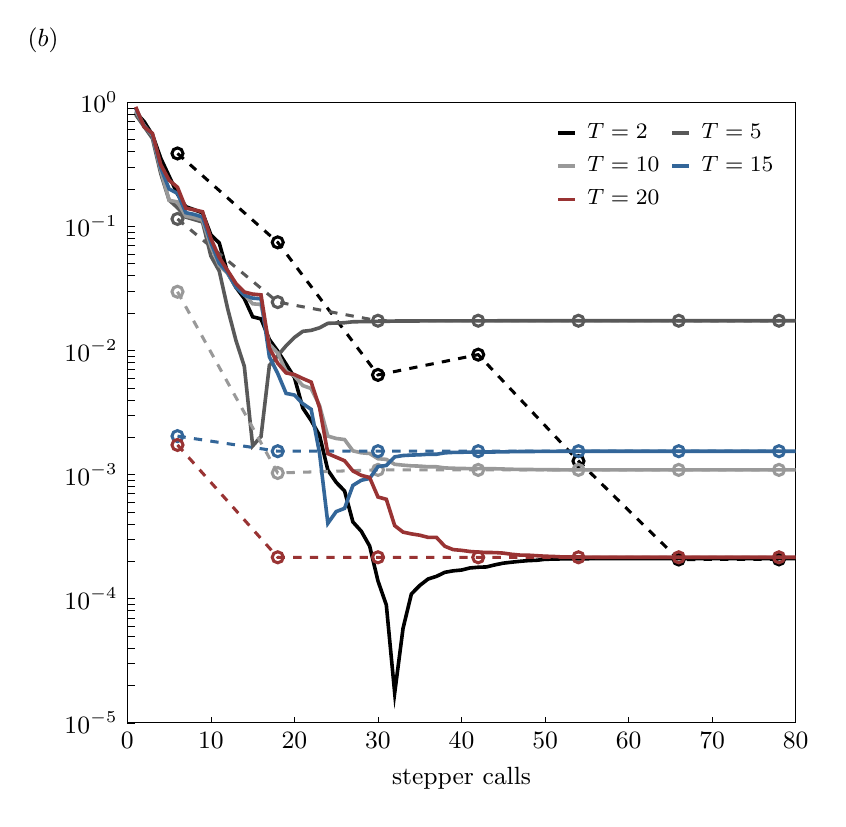
\begin{tikzpicture}

\begin{axis}[%
width=11.252in,
height=7.131in,
at={(1.887in,0.962in)},
scale only axis,
clip=true,
separate axis lines,
every outer x axis line/.append style={black},
every x tick label/.append style={font=\color{black}},
every x tick/.append style={black},
xmin=0,
xmax=80,
xlabel={stepper calls},
every outer y axis line/.append style={black},
every y tick label/.append style={font=\color{black}},
every y tick/.append style={black},
ymode=log,
ymin=1e-05,
ymax=1,
yminorticks=true,
axis background/.style={fill=white},
legend style={legend cell align=left, align=left},
clip=true,
clip mode=individual,
axis lines=box,
xtick pos=bottom,
ytick pos=left,
tick align=inside,
major tick length=2pt,
width=0.7\linewidth,
height=0.65\linewidth,
every axis/.append style={font=\fontsize{9}{9}\selectfont},xlabel style={font=\fontsize{9}{9}\selectfont},title style={font=\fontsize{9}{9}\selectfont},
legend style={font=\fontsize{8}{9}\selectfont,inner sep=1pt,row sep=1pt,column sep=2pt,nodes={scale=1.00},draw=none},legend image post style={xscale=0.35},
legend columns=2,
scaled x ticks=false,
tick label style={/pgf/number format/fixed,/pgf/number format/precision=2},
every x tick label/.append style={font=\fontsize{9}{9}\selectfont\color{black}},
every y tick label/.append style={font=\fontsize{9}{9}\selectfont\color{black}},
,,
colormap={sigmamap}{rgb(0.0000)=(0.0200,0.1880,0.3800); rgb(0.1000)=(0.0743,0.3456,0.5616); rgb(0.2000)=(0.1918,0.4980,0.7060); rgb(0.3000)=(0.3890,0.6708,0.8226); rgb(0.4000)=(0.7552,0.8682,0.9228); rgb(0.5000)=(0.9690,0.9689,0.9689); rgb(0.6000)=(0.9425,0.8044,0.7614); rgb(0.7000)=(0.8767,0.4910,0.4020); rgb(0.8000)=(0.7869,0.2866,0.2470); rgb(0.9000)=(0.6186,0.1239,0.1568); rgb(1.0000)=(0.4040,0.0000,0.1220)}
]
\addplot [color=black, line width=1.3pt]
  table[row sep=crcr]{%
1	0.832142165809318\\
2	0.698807622707636\\
3	0.546807535646839\\
4	0.353256308468127\\
5	0.2533545113672\\
6	0.181829801602638\\
7	0.143961931458514\\
8	0.136069474952372\\
9	0.128276084439533\\
10	0.0853515771514262\\
11	0.0733972032655607\\
12	0.0421167159491625\\
13	0.032179511831854\\
14	0.026197264594499\\
15	0.0186703519100572\\
16	0.0179558484860287\\
17	0.0122477491436808\\
18	0.00987930822292705\\
19	0.00776495043096266\\
20	0.00605286229772802\\
21	0.00343739612353565\\
22	0.00272330657881337\\
23	0.00207295030764483\\
24	0.00108590094293048\\
25	0.000864740726484522\\
26	0.000738121574372372\\
27	0.000414905706821819\\
28	0.00034958297313094\\
29	0.000265902270606906\\
30	0.00013885897151188\\
31	8.89550707338264e-05\\
32	1.73790854390435e-05\\
33	5.76632853457698e-05\\
34	0.000109156501001198\\
35	0.00012774614898567\\
36	0.000144046922404943\\
37	0.00015125888994871\\
38	0.000163039715967061\\
39	0.000167572474343433\\
40	0.000170111260942139\\
41	0.000176730335302363\\
42	0.000179193232154384\\
43	0.000180193469332686\\
44	0.000187283454047588\\
45	0.000193282521925197\\
46	0.000196773393056463\\
47	0.000199941632828961\\
48	0.00020259610362408\\
49	0.000203846130160141\\
50	0.000207689293072777\\
51	0.000208237218434015\\
52	0.000209155919455236\\
53	0.000209450502219311\\
54	0.000209536602094388\\
55	0.000209777778221061\\
56	0.000210214244888818\\
57	0.000210347836618805\\
58	0.000210400349410914\\
59	0.000210438042734826\\
60	0.000210494518788903\\
61	0.00021053015716279\\
62	0.000210553322293998\\
63	0.000210591647673277\\
64	0.000210600334145073\\
65	0.000210608254088011\\
66	0.000210610705413184\\
67	0.000210628975313441\\
68	0.000210638519721798\\
69	0.00021064846641863\\
70	0.000210662651566689\\
71	0.000210669744848924\\
72	0.000210670730477753\\
73	0.00021067379487986\\
74	0.00021067430095941\\
75	0.000210675244846075\\
76	0.000210678230149818\\
77	0.000210679715527429\\
78	0.000210681515133548\\
79	0.000210682541956614\\
80	0.000210683452492522\\
};
\addlegendentry{$T=2$}

\addplot [color=black, dashed, line width=1.1pt, mark size=2.0pt, mark=o, mark options={solid, black}, forget plot]
  table[row sep=crcr]{%
6	0.38634485377839\\
18	0.0742417278942887\\
30	0.00635197919233409\\
42	0.00924881520992697\\
54	0.00128367921167339\\
66	0.000206791538716321\\
78	0.000207192745182013\\
};
\addplot [color=white!35!black, line width=1.3pt]
  table[row sep=crcr]{%
1	0.794201241174241\\
2	0.636392197071579\\
3	0.511097089381333\\
4	0.265419020726859\\
5	0.162490441026057\\
6	0.141282246946287\\
7	0.118583735195212\\
8	0.113387263024999\\
9	0.108295982662846\\
10	0.0575898627114288\\
11	0.0436663052599052\\
12	0.0217657425047832\\
13	0.0120211522516976\\
14	0.0074518699460532\\
15	0.00170193007565686\\
16	0.00202554643688287\\
17	0.00758054743888711\\
18	0.00906925911452958\\
19	0.0109020267657692\\
20	0.0127229895482339\\
21	0.0142466131427801\\
22	0.014511566017313\\
23	0.0152074097413436\\
24	0.0165363359023962\\
25	0.0166275793436142\\
26	0.0167221533865549\\
27	0.017020440194329\\
28	0.017052879094671\\
29	0.0170842802529692\\
30	0.0171531143988702\\
31	0.0171705074859301\\
32	0.0172345496823139\\
33	0.0172498491050995\\
34	0.0172727133096399\\
35	0.0172784599704133\\
36	0.0172960038585485\\
37	0.0172978670507015\\
38	0.01730889148876\\
39	0.0173133715233898\\
40	0.0173157228794942\\
41	0.0173190670670061\\
42	0.0173195332858691\\
43	0.017320037760821\\
44	0.0173259167076527\\
45	0.0173337316030692\\
46	0.0173368796634658\\
47	0.0173412042420974\\
48	0.0173436768691506\\
49	0.0173448400265504\\
50	0.0173486162131316\\
51	0.0173493433608628\\
52	0.0173505716335023\\
53	0.017350966015995\\
54	0.0173510185610251\\
55	0.0173511600156901\\
56	0.0173515131306214\\
57	0.0173516525332058\\
58	0.0173516722123954\\
59	0.0173516795960179\\
60	0.0173517096502393\\
61	0.0173517359992392\\
62	0.017351744959992\\
63	0.0173517931405994\\
64	0.0173518010342846\\
65	0.0173518047589665\\
66	0.0173518054387212\\
67	0.0173518203585172\\
68	0.0173518252274636\\
69	0.0173518287235146\\
70	0.0173518399862865\\
71	0.0173518442887167\\
72	0.0173518449779994\\
73	0.0173518463888206\\
74	0.0173518466964082\\
75	0.0173518471354517\\
76	0.0173518497824039\\
77	0.0173518517715081\\
78	0.0173518530042554\\
79	0.0173518540916225\\
80	0.0173518547635486\\
};
\addlegendentry{$T=5$}

\addplot [color=white!35!black, dashed, line width=1.1pt, mark size=2.0pt, mark=o, mark options={solid, white!35!black}, forget plot]
  table[row sep=crcr]{%
6	0.114627266417663\\
18	0.0245110260665455\\
30	0.0173550749753947\\
42	0.0173553372422539\\
54	0.0173517356824942\\
66	0.017351859167501\\
78	0.0173518546728774\\
};
\addplot [color=white!60!black, line width=1.3pt]
  table[row sep=crcr]{%
1	0.84876248212394\\
2	0.649751643309823\\
3	0.540037042350577\\
4	0.281205903590061\\
5	0.161982206992004\\
6	0.157231809946868\\
7	0.120760737936852\\
8	0.117029821354168\\
9	0.112056444044837\\
10	0.0687652892723018\\
11	0.048285017579275\\
12	0.0417577423341335\\
13	0.0322687478482075\\
14	0.0282339730743595\\
15	0.0237409519465848\\
16	0.0234741596608912\\
17	0.0112296011081531\\
18	0.00950138804760071\\
19	0.00682450635838535\\
20	0.00619634569975223\\
21	0.00521017233758741\\
22	0.00493419836620897\\
23	0.00360091672537679\\
24	0.00204089843628622\\
25	0.00195294587640533\\
26	0.00191430181873946\\
27	0.00155264879828137\\
28	0.00149756666011107\\
29	0.00147789912083002\\
30	0.00134143911241692\\
31	0.00132501903343994\\
32	0.00120988481005397\\
33	0.00119044401344739\\
34	0.00117515581497276\\
35	0.00116975101375087\\
36	0.0011554929174147\\
37	0.00115496662479683\\
38	0.00113086248234519\\
39	0.00112391470680959\\
40	0.00111957803700095\\
41	0.00111600433861349\\
42	0.00111552739337057\\
43	0.00111471028631988\\
44	0.00111352913783512\\
45	0.0011081362684778\\
46	0.00110309615758645\\
47	0.00109914002544802\\
48	0.00109794609075457\\
49	0.00109669697086278\\
50	0.00109437995187906\\
51	0.00109324886331059\\
52	0.00109167301886039\\
53	0.00109121922217887\\
54	0.00109118414593429\\
55	0.00109100173467356\\
56	0.00109057373932463\\
57	0.00109051293803442\\
58	0.00109048423798858\\
59	0.00109046877807932\\
60	0.00109045447447922\\
61	0.00109041790193447\\
62	0.00109040528986774\\
63	0.0010903459823417\\
64	0.00109033486099181\\
65	0.00109033423654462\\
66	0.00109033348021297\\
67	0.00109032532582996\\
68	0.00109031228143468\\
69	0.0010903119490669\\
70	0.00109030690376152\\
71	0.00109030227805846\\
72	0.00109030126088857\\
73	0.0010902994965216\\
74	0.00109029930624357\\
75	0.00109029917664437\\
76	0.00109029842187397\\
77	0.00109029714172199\\
78	0.00109029665316491\\
79	0.00109029500376933\\
80	0.00109029460601764\\
};
\addlegendentry{$T=10$}

\addplot [color=white!60!black, dashed, line width=1.1pt, mark size=2.0pt, mark=o, mark options={solid, white!60!black}, forget plot]
  table[row sep=crcr]{%
6	0.0296986393320929\\
18	0.00102941666107282\\
30	0.00109027663329274\\
42	0.00109029472584195\\
54	0.00109029460615259\\
66	0.00109029460601256\\
78	0.00109029460601087\\
};
\addplot [color=mycolor1, line width=1.3pt]
  table[row sep=crcr]{%
1	0.894315116322509\\
2	0.639924565807262\\
3	0.550585211968434\\
4	0.29541887879764\\
5	0.19993958879838\\
6	0.184291417981773\\
7	0.128648029366811\\
8	0.12466547313007\\
9	0.118843197055609\\
10	0.0741895421110601\\
11	0.0503504136921993\\
12	0.042501822485729\\
13	0.0322887958668297\\
14	0.0278491723748038\\
15	0.0263846834294881\\
16	0.0260585377750902\\
17	0.00888618726500854\\
18	0.00652609261204634\\
19	0.00450711030892488\\
20	0.00437181197927593\\
21	0.00372419760204234\\
22	0.0033559953999986\\
23	0.00149116875713173\\
24	0.000404631592314746\\
25	0.000502966377477281\\
26	0.000534261061203403\\
27	0.000817412827319104\\
28	0.000899373545622831\\
29	0.000930054060066246\\
30	0.00115954606743714\\
31	0.00118387273760401\\
32	0.00138833905161327\\
33	0.00142293184311428\\
34	0.0014351466626162\\
35	0.00144229952283777\\
36	0.00145646421016995\\
37	0.00145681734349956\\
38	0.00149595012924684\\
39	0.00150843272503628\\
40	0.00151261330844982\\
41	0.00151757116846259\\
42	0.00151899574832936\\
43	0.00152050844936937\\
44	0.00152061485037717\\
45	0.00152373363012612\\
46	0.0015293021478584\\
47	0.00153293167946044\\
48	0.00153367078561144\\
49	0.00153544559513626\\
50	0.00153757916197315\\
51	0.00153872824909911\\
52	0.00154044556888507\\
53	0.0015409253005438\\
54	0.00154094408191749\\
55	0.00154118412931707\\
56	0.00154164954964419\\
57	0.00154166821745001\\
58	0.00154172360755486\\
59	0.0015417595257933\\
60	0.00154179792928781\\
61	0.00154183947136366\\
62	0.00154186468740169\\
63	0.00154192030448154\\
64	0.00154192879628973\\
65	0.00154192998822334\\
66	0.00154193066601282\\
67	0.00154193558818563\\
68	0.00154195816204324\\
69	0.0015419582470162\\
70	0.0015419628392149\\
71	0.00154197016611782\\
72	0.00154197165242503\\
73	0.00154197521858553\\
74	0.00154197531177196\\
75	0.00154197547382402\\
76	0.00154197565835642\\
77	0.00154197639456516\\
78	0.00154197699776023\\
79	0.0015419785909014\\
80	0.00154197898234938\\
};
\addlegendentry{$T=15$}

\addplot [color=mycolor1, dashed, line width=1.1pt, mark size=2.0pt, mark=o, mark options={solid, mycolor1}, forget plot]
  table[row sep=crcr]{%
6	0.00203990605396475\\
18	0.00154172974518009\\
30	0.0015419790075907\\
42	0.00154197898235307\\
54	0.00154197898235694\\
66	0.00154197898235731\\
78	0.00154197898235675\\
};
\addplot [color=red!60!teal, line width=1.3pt]
  table[row sep=crcr]{%
1	0.916655916931551\\
2	0.632839416655546\\
3	0.560734559075273\\
4	0.313608263459002\\
5	0.235135400577056\\
6	0.206351388400978\\
7	0.140042582106633\\
8	0.135687874596275\\
9	0.130995901556129\\
10	0.0798097946470546\\
11	0.0561312542461006\\
12	0.0440889906468997\\
13	0.0345946063616061\\
14	0.0295636019494487\\
15	0.0284412871383848\\
16	0.0280350603307864\\
17	0.0104376190014379\\
18	0.00788512184256926\\
19	0.0065903174958666\\
20	0.00639253620729769\\
21	0.00593748810345597\\
22	0.00555655425078409\\
23	0.00347899564883621\\
24	0.00147495861576603\\
25	0.00137946800118453\\
26	0.00129225679938062\\
27	0.00106924562969753\\
28	0.000985488853024056\\
29	0.00094617686728798\\
30	0.000659211687506794\\
31	0.000631845660007868\\
32	0.000387808663954991\\
33	0.00034374747666017\\
34	0.000332697949419378\\
35	0.000324602961382195\\
36	0.000311797257064023\\
37	0.000311673173719314\\
38	0.000264364495329873\\
39	0.00024839828505949\\
40	0.000245128238914654\\
41	0.000239946394987256\\
42	0.000237379566910402\\
43	0.000235452543395795\\
44	0.000235199818794693\\
45	0.000232905289889007\\
46	0.000227852328983014\\
47	0.000224513740367466\\
48	0.000223982941141446\\
49	0.000221896853141786\\
50	0.000219866449830847\\
51	0.00021881124715571\\
52	0.000217019068638015\\
53	0.00021654654148235\\
54	0.000216534858195951\\
55	0.000216288001097712\\
56	0.000215814272028608\\
57	0.000215808852322244\\
58	0.000215741855002887\\
59	0.000215693082893171\\
60	0.000215631590872829\\
61	0.000215585983924185\\
62	0.000215548556690648\\
63	0.000215499396187992\\
64	0.000215493962406096\\
65	0.000215491597973077\\
66	0.000215490951095293\\
67	0.000215484732640243\\
68	0.000215460459439456\\
69	0.000215460355978811\\
70	0.00021545544417535\\
71	0.00021544709332156\\
72	0.000215445458395092\\
73	0.000215440651942681\\
74	0.000215440608018712\\
75	0.0002154403656884\\
76	0.000215440280989658\\
77	0.000215439759644969\\
78	0.000215438987861761\\
79	0.000215437625663258\\
80	0.000215437213033184\\
};
\addlegendentry{$T=20$}

\addplot [color=red!60!teal, dashed, line width=1.1pt, mark size=2.0pt, mark=o, mark options={solid, red!60!teal}, forget plot]
  table[row sep=crcr]{%
6	0.00173146060343864\\
18	0.000215427460460972\\
30	0.000215437213018904\\
42	0.000215437213023171\\
54	0.000215437213029573\\
66	0.000215437213026782\\
78	0.000215437213026126\\
};
\node[right, align=left, inner sep=0]
at (rel axis cs:-0.15,1.1) {$(b)$};
\end{axis}
\end{tikzpicture}%
    \end{minipage}
    \caption{Ginzburg--Landau relative error versus stepper calls for \((a)\) slow and \((b)\) fast covariance-spectrum decay. (\solidlegend) deterministic truncation; (\dashlegend\circlegend) SSTE; dotted line: \(\epsilon_{\mathrm{rel}}=10^{-2}\).}
    \label{fig:GL_eig_vs_sste}
\end{figure}
We compare the cost of SSTE against the deterministic truncation strategy on the linear complex Ginzburg--Landau system used in the numerical experiments. As discussed by \citet{frame-towne-2024}, this model provides a useful canonical setting for transient-growth and time-stepping studies. In continuous form, the governing equation is
\begin{equation}
  \frac{\partial q}{\partial t}
  =
  -\nu\frac{\partial q}{\partial x}
  +
  \gamma\frac{\partial^2 q}{\partial x^2}
  +
  \mu(x)q,
  \label{eq:GL_continuous_equation_sste_necessity}
\end{equation}
where \(q(x,t)\) is a complex amplitude, \(\nu\) is the convection coefficient, \(\gamma\) is the complex diffusion coefficient, and \(\mu(x)\) is a spatially varying growth-rate profile. In the present computations, the latter is taken in quadratic form,
\begin{equation}
  \mu(x)
  =
  \mu_0+\mu_2x^2,
  \label{eq:GL_mu_profile_sste_necessity}
\end{equation}
with parameter values
\begin{equation}
  \nu = 2+0.4\mathrm{i},
  \qquad
  \gamma = 1-\mathrm{i},
  \qquad
  \mu_2 = -0.01,
  \qquad
  \mu_0 = 0.39.
  \label{eq:GL_parameters_sste_necessity}
\end{equation}
We use \(n_x=80\), \(\Delta t=0.08\), and \(2\leq T\leq20\); higher-order Hermite discretizations are poorly conditioned.
The initial covariance is generated through
\begin{equation}
  \mathsfbi{C}_{00}^{z}
  =
  \mathsfbi{Q}
  \operatorname{diag}
  \left(
    \lambda_1,\dots,\lambda_n
  \right)
  \mathsfbi{Q}^{*},
  \label{eq:GL_covariance_construction_sste_necessity}
\end{equation}
where \(\mathsfbi{Q}\) is a fixed orthonormal basis and the eigenvalues \(\lambda_j\) are chosen to impose a prescribed spectral decay. We consider two representative cases. The first is a slow algebraic decay,
\begin{equation}
  \lambda_j
  \propto
  j^{-1/10},
  \label{eq:GL_slow_covariance_decay}
\end{equation}
and the second is a fast exponential decay,
\begin{equation}
  \lambda_j
  \propto
  \exp
  \left[
    -0.25(j-1)
  \right].
  \label{eq:GL_fast_covariance_decay}
\end{equation}
Both spectra have the same total variance. The slow case is deliberately near-flat and full-rank, delaying deterministic convergence until most of the 80 directions are propagated.

\subsubsection{Plane Poiseuille flow}
\label{sec:appendix_verification_poiseuille}
\begin{figure}[t]
    \centering
    \begin{minipage}[t]{0.48\textwidth}
        \centering
        \vspace{0pt}
        % This file was created by matlab2tikz.
%
\definecolor{mycolor1}{rgb}{0.20000,0.40000,0.60000}%
%
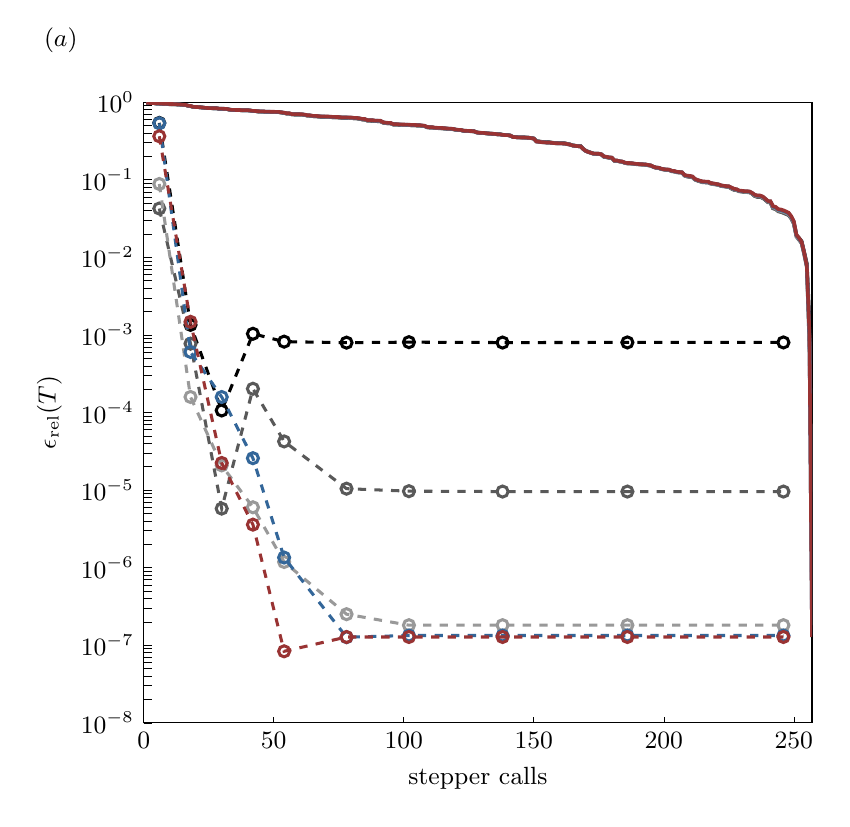
\begin{tikzpicture}

\begin{axis}[%
width=11.252in,
height=7.131in,
at={(1.887in,0.962in)},
scale only axis,
clip=true,
separate axis lines,
every outer x axis line/.append style={black},
every x tick label/.append style={font=\color{black}},
every x tick/.append style={black},
xmin=0,
xmax=257,
xlabel={stepper calls},
every outer y axis line/.append style={black},
every y tick label/.append style={font=\color{black}},
every y tick/.append style={black},
ymode=log,
ymin=1e-08,
ymax=1,
yminorticks=true,
ylabel={$\epsilon_{\mathrm{rel}}(T)$},
axis background/.style={fill=white},
clip=true,
clip mode=individual,
axis lines=box,
xtick pos=bottom,
ytick pos=left,
tick align=inside,
major tick length=2pt,
width=0.7\linewidth,
height=0.65\linewidth,
every axis/.append style={font=\fontsize{9}{9}\selectfont},xlabel style={font=\fontsize{9}{9}\selectfont},title style={font=\fontsize{9}{9}\selectfont},
legend style={font=\fontsize{8}{9}\selectfont,inner sep=1pt,row sep=1pt,column sep=2pt,nodes={scale=1.00},draw=none},legend image post style={xscale=0.35},
legend columns=1,
scaled x ticks=false,
tick label style={/pgf/number format/fixed,/pgf/number format/precision=2},
every x tick label/.append style={font=\fontsize{9}{9}\selectfont\color{black}},
every y tick label/.append style={font=\fontsize{9}{9}\selectfont\color{black}},
,,
colormap={sigmamap}{rgb(0.0000)=(0.0200,0.1880,0.3800); rgb(0.1000)=(0.0743,0.3456,0.5616); rgb(0.2000)=(0.1918,0.4980,0.7060); rgb(0.3000)=(0.3890,0.6708,0.8226); rgb(0.4000)=(0.7552,0.8682,0.9228); rgb(0.5000)=(0.9690,0.9689,0.9689); rgb(0.6000)=(0.9425,0.8044,0.7614); rgb(0.7000)=(0.8767,0.4910,0.4020); rgb(0.8000)=(0.7869,0.2866,0.2470); rgb(0.9000)=(0.6186,0.1239,0.1568); rgb(1.0000)=(0.4040,0.0000,0.1220)}
]
\addplot [color=black, line width=1.3pt, forget plot]
  table[row sep=crcr]{%
1	0.982966330608578\\
2	0.97604883720077\\
3	0.972269958891538\\
4	0.970503289638935\\
5	0.958721405225083\\
6	0.957618750114593\\
7	0.949409965780001\\
8	0.946631301384151\\
9	0.943171012824689\\
10	0.941395877849633\\
11	0.940290265059246\\
12	0.938680845066753\\
13	0.933745419964527\\
14	0.930398404968719\\
15	0.922469639890038\\
16	0.920422703961159\\
17	0.899687438112519\\
18	0.890297123781761\\
19	0.86969413750324\\
20	0.865349827896549\\
21	0.863113422223451\\
22	0.856767046091549\\
23	0.84879289854553\\
24	0.840831855227552\\
25	0.837942514843372\\
26	0.837238991301756\\
27	0.835937564003596\\
28	0.834883569615981\\
29	0.821679151704008\\
30	0.821641156782489\\
31	0.819587506270877\\
32	0.815963187418029\\
33	0.800080935248923\\
34	0.792732055253705\\
35	0.791347539085762\\
36	0.789765437092575\\
37	0.789171658957207\\
38	0.785660559843496\\
39	0.785257112321728\\
40	0.785097583433237\\
41	0.778586531726282\\
42	0.768184102914871\\
43	0.766969040934379\\
44	0.758926927712864\\
45	0.756396495819457\\
46	0.755374614863844\\
47	0.74950069971379\\
48	0.748573883440318\\
49	0.747114265567734\\
50	0.746920553620366\\
51	0.74381281171101\\
52	0.743470394194\\
53	0.734622775759791\\
54	0.725486251213745\\
55	0.712441438373767\\
56	0.712120976527085\\
57	0.695902684640726\\
58	0.69471188185694\\
59	0.694228151426545\\
60	0.693348470801481\\
61	0.691123211794459\\
62	0.683595567934903\\
63	0.670517708929653\\
64	0.669396278255485\\
65	0.659972844110037\\
66	0.659284011573087\\
67	0.654108239315489\\
68	0.648872022132782\\
69	0.647004651894603\\
70	0.646898315315815\\
71	0.645320035064132\\
72	0.641495156999121\\
73	0.638336522912256\\
74	0.636245270124167\\
75	0.63561283511298\\
76	0.630013905355875\\
77	0.629300933483904\\
78	0.629273608383272\\
79	0.626588102812313\\
80	0.6249785610807\\
81	0.618051779287091\\
82	0.61760161399641\\
83	0.610116289153122\\
84	0.598733061118022\\
85	0.596754701744156\\
86	0.578336557744394\\
87	0.577520095902458\\
88	0.57668039214578\\
89	0.569192866936287\\
90	0.568684616196599\\
91	0.567781390196765\\
92	0.545174934342963\\
93	0.537206580369471\\
94	0.534168567143395\\
95	0.531660070357362\\
96	0.515279920603679\\
97	0.515160316290744\\
98	0.51217502354736\\
99	0.510102845790237\\
100	0.508441823338196\\
101	0.507293324179209\\
102	0.50625248442349\\
103	0.504533478349842\\
104	0.50418367932901\\
105	0.50101186912038\\
106	0.500475996711498\\
107	0.495556169726679\\
108	0.491526093163103\\
109	0.474939220277814\\
110	0.471976517209076\\
111	0.471397729050771\\
112	0.464951351514588\\
113	0.462909553414059\\
114	0.462755087835895\\
115	0.459685754382438\\
116	0.456650219837631\\
117	0.4533773073742\\
118	0.45239030088586\\
119	0.448771128351402\\
120	0.441373111119473\\
121	0.437878899357908\\
122	0.436567986771897\\
123	0.42766600490534\\
124	0.426962658684734\\
125	0.424411307266562\\
126	0.423093294104886\\
127	0.421487056457706\\
128	0.40845747323444\\
129	0.403086637641859\\
130	0.402033847441137\\
131	0.39963805823747\\
132	0.395906034136358\\
133	0.393585528707658\\
134	0.391587290882353\\
135	0.390649900206814\\
136	0.386536948297603\\
137	0.38607559989746\\
138	0.380611582691387\\
139	0.378319261067495\\
140	0.377583277377092\\
141	0.371470401535299\\
142	0.356947519756303\\
143	0.355342294240175\\
144	0.352648624936454\\
145	0.352217842979882\\
146	0.351991646559007\\
147	0.350450262027681\\
148	0.348728664558269\\
149	0.34495729136732\\
150	0.340417054042536\\
151	0.314960478632387\\
152	0.31224391750994\\
153	0.30858129443841\\
154	0.307276851922746\\
155	0.304599755220858\\
156	0.304382343507257\\
157	0.300892308138577\\
158	0.298336980594795\\
159	0.297890704814015\\
160	0.297098357212825\\
161	0.296242533695882\\
162	0.294960908507088\\
163	0.289463715265222\\
164	0.284838137674088\\
165	0.277855806654834\\
166	0.274504727859216\\
167	0.272738580449843\\
168	0.271597079745049\\
169	0.250008657723613\\
170	0.236175429837658\\
171	0.229519436480829\\
172	0.223306566476213\\
173	0.217704853889386\\
174	0.217075226705583\\
175	0.216849872756759\\
176	0.212100689986535\\
177	0.197922224306309\\
178	0.195473806039263\\
179	0.192569664433095\\
180	0.191886950398255\\
181	0.176321829335418\\
182	0.176204493054979\\
183	0.172463392607111\\
184	0.170621903239322\\
185	0.165314988403719\\
186	0.162816088242698\\
187	0.162526474650984\\
188	0.161678528039627\\
189	0.159804474035487\\
190	0.158932133711831\\
191	0.157800302896849\\
192	0.157306968318194\\
193	0.156737123015743\\
194	0.153987930466226\\
195	0.152326731562892\\
196	0.146403680036494\\
197	0.143332220703391\\
198	0.142404957423671\\
199	0.138318017143347\\
200	0.136175805378474\\
201	0.134661682318101\\
202	0.13436358968688\\
203	0.129508102469386\\
204	0.128403683267132\\
205	0.12543655257506\\
206	0.124809848549587\\
207	0.124055903093489\\
208	0.113575556045366\\
209	0.110608590113858\\
210	0.109552532273075\\
211	0.107969507101389\\
212	0.101027338240515\\
213	0.097803717398423\\
214	0.0955306143288746\\
215	0.0932514775609851\\
216	0.0930263447886719\\
217	0.0929092471308039\\
218	0.0899489553254883\\
219	0.0886650201623336\\
220	0.0877413646642759\\
221	0.0864065450407232\\
222	0.0838469939164371\\
223	0.0830610312376052\\
224	0.0820146517143478\\
225	0.0813842215555414\\
226	0.077576766810229\\
227	0.0745877437127478\\
228	0.0738979308037943\\
229	0.0716342426149204\\
230	0.0709763409928529\\
231	0.0699835156519321\\
232	0.0699233608336728\\
233	0.0693814538777797\\
234	0.0663670778628009\\
235	0.0618109747664514\\
236	0.0603545842356326\\
237	0.0603415309260477\\
238	0.0584113841832503\\
239	0.0556902643722308\\
240	0.0517211154263843\\
241	0.0511581131244168\\
242	0.0430304290108372\\
243	0.0421833016960384\\
244	0.0395771986799776\\
245	0.0388023074808236\\
246	0.0376868444208258\\
247	0.0364514261558841\\
248	0.0353058581982174\\
249	0.0321373391485221\\
250	0.0275465832028203\\
251	0.0192319951327931\\
252	0.0177656087315\\
253	0.0160570296940422\\
254	0.011589220689924\\
255	0.00827908511913625\\
256	0.00148125784234795\\
257	0.000799887133449348\\
};
\addplot [color=black, dashed, line width=1.1pt, mark size=2.0pt, mark=o, mark options={solid, black}, forget plot]
  table[row sep=crcr]{%
6	0.540776137824498\\
18	0.00134857593831537\\
30	0.000106169089263514\\
42	0.00103472753047721\\
54	0.000818869801991856\\
78	0.000795027686100323\\
102	0.00080652247982178\\
138	0.000797136215325989\\
186	0.000799978080205416\\
246	0.000799887317381151\\
};
\addplot [color=white!35!black, line width=1.3pt, forget plot]
  table[row sep=crcr]{%
1	0.983721731500279\\
2	0.976660572325747\\
3	0.972839765959342\\
4	0.971301944669699\\
5	0.959799388973549\\
6	0.958845785394696\\
7	0.950915762436377\\
8	0.948041225904038\\
9	0.944346971973855\\
10	0.942540613520157\\
11	0.94138602620319\\
12	0.939761896169868\\
13	0.934356346896206\\
14	0.931111268656859\\
15	0.923302424930562\\
16	0.921478664417873\\
17	0.899741624448408\\
18	0.890432187571784\\
19	0.869300494849979\\
20	0.865058581388375\\
21	0.862798872541602\\
22	0.856474746027135\\
23	0.848536004128235\\
24	0.840371331165609\\
25	0.837276405728466\\
26	0.836594436298206\\
27	0.835141284275067\\
28	0.834298718469335\\
29	0.821337155438688\\
30	0.821295692243148\\
31	0.819295008323054\\
32	0.815413158213949\\
33	0.79952914798548\\
34	0.792159017364284\\
35	0.790726732613222\\
36	0.789309976737867\\
37	0.78871132463182\\
38	0.785295804424289\\
39	0.784868817221122\\
40	0.784665853107149\\
41	0.778426668236252\\
42	0.767800574043802\\
43	0.766544033207126\\
44	0.758861657858685\\
45	0.756266684319795\\
46	0.755297466880924\\
47	0.749736860798518\\
48	0.748832270444804\\
49	0.747316222540201\\
50	0.747124160165675\\
51	0.743815661846753\\
52	0.74352402584819\\
53	0.734804186102495\\
54	0.726012073172219\\
55	0.713160171571788\\
56	0.712819168031805\\
57	0.696035404032751\\
58	0.694899194569886\\
59	0.694452784105282\\
60	0.693545123847677\\
61	0.691468075089052\\
62	0.683859289397706\\
63	0.670697255063324\\
64	0.669618074520227\\
65	0.659894134355704\\
66	0.659257138344594\\
67	0.654192946539639\\
68	0.649121825806224\\
69	0.647377004423068\\
70	0.647257749951999\\
71	0.645637324810665\\
72	0.641644297563263\\
73	0.638644926606291\\
74	0.636659888389678\\
75	0.636016696380125\\
76	0.630442991047505\\
77	0.629691127532882\\
78	0.629663571456078\\
79	0.626962015004404\\
80	0.625303929218444\\
81	0.618518590554813\\
82	0.618136407226562\\
83	0.610763401580046\\
84	0.599703852657755\\
85	0.597767926376595\\
86	0.579307343374107\\
87	0.578556908511256\\
88	0.577775110223124\\
89	0.570280511409948\\
90	0.569645275139811\\
91	0.568672815433737\\
92	0.545940826157171\\
93	0.537489471573664\\
94	0.534622988925008\\
95	0.53196759861026\\
96	0.515165461570201\\
97	0.515059546573259\\
98	0.512015654184668\\
99	0.509984678533576\\
100	0.508322690590231\\
101	0.507173934668139\\
102	0.505891996014098\\
103	0.504161690246267\\
104	0.503836246353716\\
105	0.500755667095347\\
106	0.500148189553613\\
107	0.495232399677385\\
108	0.490992829688539\\
109	0.47444739476465\\
110	0.471364808374564\\
111	0.470852558846438\\
112	0.46402871467548\\
113	0.462129610430649\\
114	0.461934175426679\\
115	0.458858161668526\\
116	0.455926172006135\\
117	0.45239406251629\\
118	0.451405565888917\\
119	0.447739464588823\\
120	0.440197321956762\\
121	0.436709575562376\\
122	0.435369708156115\\
123	0.426486648442205\\
124	0.425768117268333\\
125	0.423295217565363\\
126	0.422069531227627\\
127	0.42042549594331\\
128	0.407182141326848\\
129	0.401976405552608\\
130	0.400983187764168\\
131	0.398802595546109\\
132	0.395141527383881\\
133	0.392762339182165\\
134	0.390518532446232\\
135	0.389605097450214\\
136	0.385188083104472\\
137	0.384738975160471\\
138	0.379129008690447\\
139	0.376921521850993\\
140	0.376061413808015\\
141	0.36998203054877\\
142	0.355684850507635\\
143	0.354064865128139\\
144	0.351380734335976\\
145	0.351012165164004\\
146	0.35079893919004\\
147	0.349273321309767\\
148	0.347519892386844\\
149	0.343947425478915\\
150	0.33925139899578\\
151	0.312776128560529\\
152	0.310061507704277\\
153	0.306345270919523\\
154	0.305119137125808\\
155	0.302424694587555\\
156	0.302228278258648\\
157	0.298976198549163\\
158	0.296447995791092\\
159	0.295975825222196\\
160	0.295207626119482\\
161	0.294301927680087\\
162	0.293193725519402\\
163	0.287807795861337\\
164	0.283371540934813\\
165	0.276144097437816\\
166	0.272913117956184\\
167	0.270969306791585\\
168	0.269810561212348\\
169	0.24831889256419\\
170	0.234361131190009\\
171	0.227591528571758\\
172	0.22169980762679\\
173	0.216046146159817\\
174	0.21553423309152\\
175	0.215277881870524\\
176	0.211039071269715\\
177	0.197209807991937\\
178	0.194842712537043\\
179	0.191786914851731\\
180	0.191000872839168\\
181	0.175555094863494\\
182	0.17541158351594\\
183	0.171679137315959\\
184	0.169957135630688\\
185	0.164699124574965\\
186	0.162299552708448\\
187	0.162032621884314\\
188	0.161045389626439\\
189	0.159113085063453\\
190	0.158212445369588\\
191	0.157121746924538\\
192	0.156609347346084\\
193	0.156058045476637\\
194	0.153399999616301\\
195	0.151714045363992\\
196	0.145689946537044\\
197	0.142333898656792\\
198	0.141511082028109\\
199	0.137248939827936\\
200	0.135154630010122\\
201	0.133792968433812\\
202	0.133480603711473\\
203	0.128739464224185\\
204	0.12758439541454\\
205	0.124594275787022\\
206	0.123812912840757\\
207	0.12294785729522\\
208	0.11282879460601\\
209	0.110043883983169\\
210	0.109072275811829\\
211	0.107451659079384\\
212	0.100326949657664\\
213	0.0971007378046024\\
214	0.0949502053810914\\
215	0.0925531958522484\\
216	0.0923145226876021\\
217	0.0921888158672689\\
218	0.0890373140921958\\
219	0.0877737359853838\\
220	0.0867448467395237\\
221	0.0855261552854014\\
222	0.0830294432371949\\
223	0.0821235807980739\\
224	0.0811546294500055\\
225	0.0805359064013733\\
226	0.0769383803051045\\
227	0.0740384553315421\\
228	0.0732644994468261\\
229	0.0708651061704157\\
230	0.0702382799068362\\
231	0.0693089736284029\\
232	0.0692472339575829\\
233	0.068615548551236\\
234	0.0658212553165535\\
235	0.0615423709681331\\
236	0.0601802785121967\\
237	0.0601565782594766\\
238	0.0582951298019207\\
239	0.0553340172415406\\
240	0.0512981201613456\\
241	0.050804381136601\\
242	0.0427730740333626\\
243	0.0418490418795195\\
244	0.0391742378748484\\
245	0.0384458175943264\\
246	0.0373723632556348\\
247	0.0361811635809749\\
248	0.0349470450914869\\
249	0.0316221908211703\\
250	0.0270292946524804\\
251	0.0184742093757056\\
252	0.0167652606864055\\
253	0.0151053150621221\\
254	0.0108364747434359\\
255	0.00745626623942512\\
256	0.000740077970959662\\
257	9.5638055352644e-06\\
};
\addplot [color=white!35!black, dashed, line width=1.1pt, mark size=2.0pt, mark=o, mark options={solid, white!35!black}, forget plot]
  table[row sep=crcr]{%
6	0.0425726702224608\\
18	0.000771103631284935\\
30	5.76953839186773e-06\\
42	0.000202269655849491\\
54	4.23633235146686e-05\\
78	1.04201734344765e-05\\
102	9.67580865857114e-06\\
138	9.56323720505195e-06\\
186	9.56385438447046e-06\\
246	9.56380553744547e-06\\
};
\addplot [color=white!60!black, line width=1.3pt, forget plot]
  table[row sep=crcr]{%
1	0.984438196041516\\
2	0.977250889648189\\
3	0.973538493665872\\
4	0.972148413672703\\
5	0.961423255261589\\
6	0.960612714763109\\
7	0.953107091090466\\
8	0.950137039255104\\
9	0.946412008453305\\
10	0.944533892675864\\
11	0.943321070645482\\
12	0.941737052353571\\
13	0.935695871106321\\
14	0.932460740045847\\
15	0.924767228785686\\
16	0.92313703400658\\
17	0.90062716364848\\
18	0.891501706078173\\
19	0.869638793498805\\
20	0.8654779956666\\
21	0.86325844878803\\
22	0.857115601289254\\
23	0.84932205742142\\
24	0.841035860613004\\
25	0.837665480488096\\
26	0.83695350630032\\
27	0.835391985009747\\
28	0.834743232211089\\
29	0.822335686089452\\
30	0.822301185753557\\
31	0.820254611640779\\
32	0.816190336478491\\
33	0.800397102494706\\
34	0.793158896356638\\
35	0.791676728111207\\
36	0.790352938215864\\
37	0.789762860283539\\
38	0.786480983312684\\
39	0.786049064116082\\
40	0.785784931736868\\
41	0.779768185955226\\
42	0.768917697806536\\
43	0.767619499987759\\
44	0.760549230896024\\
45	0.757906960883045\\
46	0.756961630810407\\
47	0.751725870175965\\
48	0.750876000381561\\
49	0.74938229640779\\
50	0.749167114182767\\
51	0.745710591379976\\
52	0.745448345492567\\
53	0.737000677068402\\
54	0.728474359858584\\
55	0.715816734997077\\
56	0.715488433371106\\
57	0.698245694043465\\
58	0.697147951172875\\
59	0.696815944938359\\
60	0.695851276611026\\
61	0.693901924020054\\
62	0.686342534755478\\
63	0.673477326207909\\
64	0.672413996437189\\
65	0.662493941968813\\
66	0.661943474750917\\
67	0.656974357751622\\
68	0.652060813851287\\
69	0.650363623729753\\
70	0.650230757616197\\
71	0.648570424500669\\
72	0.644464350084388\\
73	0.641634077075451\\
74	0.639716488977034\\
75	0.639098013133221\\
76	0.633564825552144\\
77	0.632806637693438\\
78	0.632776550301435\\
79	0.630219953325068\\
80	0.6285708404064\\
81	0.621986233148742\\
82	0.621668453414749\\
83	0.614192848184915\\
84	0.603543736133059\\
85	0.601669208031684\\
86	0.582932989772586\\
87	0.582286403322812\\
88	0.581512908065036\\
89	0.573952430093363\\
90	0.573139861399523\\
91	0.57209301972925\\
92	0.549103064089356\\
93	0.54033116477838\\
94	0.537577968940599\\
95	0.534915347241\\
96	0.517616901939132\\
97	0.517510809643035\\
98	0.514522911031465\\
99	0.512563753520298\\
100	0.51095934474651\\
101	0.509812722419265\\
102	0.508199748534845\\
103	0.506433159136401\\
104	0.506115569764798\\
105	0.503014449648495\\
106	0.502329747679228\\
107	0.497637009916537\\
108	0.493165216820319\\
109	0.476377079194557\\
110	0.473122492268175\\
111	0.472685148938307\\
112	0.465691811942206\\
113	0.463867352465157\\
114	0.463609502935609\\
115	0.460618049109904\\
116	0.45777893861093\\
117	0.45404316895493\\
118	0.45300442944444\\
119	0.449400474349613\\
120	0.441498328011525\\
121	0.437897702841981\\
122	0.436533108068428\\
123	0.427400020490414\\
124	0.426577349100371\\
125	0.424238488406351\\
126	0.42304493184229\\
127	0.42129500581268\\
128	0.407733754124686\\
129	0.402654198527134\\
130	0.401633639134831\\
131	0.399591756914907\\
132	0.395978191742509\\
133	0.39349350552974\\
134	0.391049197418753\\
135	0.390162295741211\\
136	0.385401729792171\\
137	0.384903159989808\\
138	0.379140019772928\\
139	0.377020153547278\\
140	0.376069270322217\\
141	0.370188593224544\\
142	0.355990483916006\\
143	0.354338771145094\\
144	0.35152189727626\\
145	0.351174905869468\\
146	0.350971969632866\\
147	0.34943728555485\\
148	0.347614029527348\\
149	0.344316925450285\\
150	0.339589430361029\\
151	0.31200244779414\\
152	0.309349513623591\\
153	0.305599118283937\\
154	0.304490752736916\\
155	0.301817861873773\\
156	0.301613212636632\\
157	0.298830274524587\\
158	0.296209518035964\\
159	0.295711681745862\\
160	0.294908794975138\\
161	0.293987690196305\\
162	0.29302567247614\\
163	0.287781366912243\\
164	0.283483767268958\\
165	0.276078772779\\
166	0.273024521850267\\
167	0.270860292779637\\
168	0.26963627986392\\
169	0.24878026495233\\
170	0.234663904031939\\
171	0.227625376320666\\
172	0.222048459659075\\
173	0.216426018521787\\
174	0.215956378299498\\
175	0.215649679586962\\
176	0.211832137828534\\
177	0.198379916166883\\
178	0.196041223667668\\
179	0.192831703145837\\
180	0.191922116616984\\
181	0.176283371394621\\
182	0.176123960411809\\
183	0.17240105608116\\
184	0.170792278019413\\
185	0.165513729176464\\
186	0.163255797306021\\
187	0.163019596586466\\
188	0.161906219225444\\
189	0.159869397011314\\
190	0.158983100137573\\
191	0.157926242709283\\
192	0.157351962738762\\
193	0.156762067413474\\
194	0.154242565931781\\
195	0.152413185728589\\
196	0.146447092608558\\
197	0.142796630104112\\
198	0.142091969748519\\
199	0.137818322954891\\
200	0.135667532177481\\
201	0.134455206141531\\
202	0.134118431059526\\
203	0.129495223557602\\
204	0.128341356051089\\
205	0.125389329104555\\
206	0.124446816815473\\
207	0.123515257270778\\
208	0.113668762799612\\
209	0.111215702833093\\
210	0.110275861221697\\
211	0.10859704427882\\
212	0.101191039165533\\
213	0.0979610317117518\\
214	0.0958271902795158\\
215	0.0934967273819717\\
216	0.0932187566098985\\
217	0.0930894329309905\\
218	0.0897343556271128\\
219	0.0885532491878702\\
220	0.0873821287136454\\
221	0.0862683575198378\\
222	0.0837680736032251\\
223	0.0827345169872991\\
224	0.0818125387952693\\
225	0.0812705140289651\\
226	0.0779686836325485\\
227	0.0750624213772202\\
228	0.0742069811382484\\
229	0.0715578663909939\\
230	0.0710022322983575\\
231	0.0701770196729075\\
232	0.0701255086579608\\
233	0.0693857139429908\\
234	0.0666911203793207\\
235	0.0627521722941033\\
236	0.0614352276051345\\
237	0.0613958389125091\\
238	0.0595915114672801\\
239	0.0562807018656572\\
240	0.052245665098149\\
241	0.0518373984863463\\
242	0.0439786944431006\\
243	0.0429853017281701\\
244	0.0402388125541034\\
245	0.039614055313959\\
246	0.0385837413106389\\
247	0.0373770466608731\\
248	0.0360533616938746\\
249	0.0325465516189133\\
250	0.0279032988140638\\
251	0.0189491124805734\\
252	0.0170987124454109\\
253	0.015374038065023\\
254	0.011135449353681\\
255	0.00764530793416698\\
256	0.000876771473112565\\
257	1.81205973380823e-07\\
};
\addplot [color=white!60!black, dashed, line width=1.1pt, mark size=2.0pt, mark=o, mark options={solid, white!60!black}, forget plot]
  table[row sep=crcr]{%
6	0.0882449204147932\\
18	0.000158546263894275\\
30	2.08026673424925e-05\\
42	5.99655533441666e-06\\
54	1.18271275381314e-06\\
78	2.51119372926873e-07\\
102	1.81122582715968e-07\\
138	1.81205705172834e-07\\
186	1.81205973621476e-07\\
246	1.8120597277919e-07\\
};
\addplot [color=mycolor1, line width=1.3pt, forget plot]
  table[row sep=crcr]{%
1	0.984979046555728\\
2	0.977762344004689\\
3	0.97422401229873\\
4	0.972884323185155\\
5	0.96292101771676\\
6	0.96221221502663\\
7	0.95507705901735\\
8	0.95204147921312\\
9	0.948398477070442\\
10	0.946491555842803\\
11	0.945238564051925\\
12	0.943691161494871\\
13	0.937169556810045\\
14	0.933869692225292\\
15	0.926183218351588\\
16	0.924651961028707\\
17	0.901834364874588\\
18	0.892870704900758\\
19	0.870339965364721\\
20	0.866226465999293\\
21	0.864120420075511\\
22	0.858142792076508\\
23	0.850569104298476\\
24	0.842224706742624\\
25	0.838619107958216\\
26	0.837853191711839\\
27	0.836238969994582\\
28	0.835667104456301\\
29	0.82372614104189\\
30	0.82369652070334\\
31	0.821573882421239\\
32	0.817409367389452\\
33	0.801808125178607\\
34	0.794683038345624\\
35	0.793181382670936\\
36	0.791818234478965\\
37	0.791243373231866\\
38	0.788054360831366\\
39	0.787633855577587\\
40	0.787314953936164\\
41	0.7813942862848\\
42	0.770451948979776\\
43	0.769145671081232\\
44	0.762547957028142\\
45	0.759848507579816\\
46	0.758896491276212\\
47	0.75373735398808\\
48	0.752926393580488\\
49	0.751474420510401\\
50	0.751224684931217\\
51	0.74768682190135\\
52	0.747432045065007\\
53	0.739215153579631\\
54	0.730741856624636\\
55	0.718251744097016\\
56	0.717945160103779\\
57	0.700475592877424\\
58	0.699400408800778\\
59	0.699148654996058\\
60	0.698141474989377\\
61	0.696235321372734\\
62	0.688724467762319\\
63	0.676295194163577\\
64	0.675226318290551\\
65	0.665131571982671\\
66	0.664644140202097\\
67	0.659722433671249\\
68	0.654818228942684\\
69	0.653153817850148\\
70	0.653007641941007\\
71	0.651302051787327\\
72	0.647171360157201\\
73	0.644428665952818\\
74	0.642533930379262\\
75	0.641944709879106\\
76	0.636358546322258\\
77	0.635620410323294\\
78	0.635589002573583\\
79	0.633230428423561\\
80	0.631566352721277\\
81	0.625105356934239\\
82	0.624819433926981\\
83	0.617193423369116\\
84	0.606761561087893\\
85	0.604942077515237\\
86	0.585910737120139\\
87	0.585354755763201\\
88	0.584558113129068\\
89	0.57690954610101\\
90	0.575962073984441\\
91	0.574876078457187\\
92	0.551679474045353\\
93	0.54277775514811\\
94	0.540085586282079\\
95	0.537518566703271\\
96	0.519938485078341\\
97	0.519820133341328\\
98	0.516958080447775\\
99	0.515059595902115\\
100	0.513472502000987\\
101	0.512356171007906\\
102	0.510461430657877\\
103	0.508644578583082\\
104	0.508304201583455\\
105	0.505101532669923\\
106	0.5043806645722\\
107	0.499942508568545\\
108	0.495333663902341\\
109	0.478302757850775\\
110	0.474921376942366\\
111	0.474528430990486\\
112	0.467586367565165\\
113	0.465793435489065\\
114	0.465467953046149\\
115	0.462568208964251\\
116	0.459797928202949\\
117	0.455964773777906\\
118	0.454869797625158\\
119	0.45130971303161\\
120	0.443041974238248\\
121	0.439311926695577\\
122	0.437954179702021\\
123	0.428430028009257\\
124	0.427524541704305\\
125	0.425293750091169\\
126	0.424101137941698\\
127	0.42227032662227\\
128	0.408469047332927\\
129	0.403448330541981\\
130	0.402371704887521\\
131	0.400358585849785\\
132	0.396735912596379\\
133	0.394188652681824\\
134	0.391613935666266\\
135	0.390719507989045\\
136	0.385689956717372\\
137	0.385120312857692\\
138	0.379219669216968\\
139	0.377155557595791\\
140	0.376167328700289\\
141	0.370478188334312\\
142	0.356225269152565\\
143	0.354572441223781\\
144	0.351623697580591\\
145	0.351273355101006\\
146	0.351088957635978\\
147	0.349536220169029\\
148	0.347665807773466\\
149	0.344560084985144\\
150	0.339891398283475\\
151	0.311607784935495\\
152	0.308997170972734\\
153	0.305273260268609\\
154	0.304262235409794\\
155	0.301624640061336\\
156	0.301381844461452\\
157	0.298981738642644\\
158	0.29621966436292\\
159	0.295712339725817\\
160	0.294858147616419\\
161	0.293945455038766\\
162	0.293051717217513\\
163	0.287940587214346\\
164	0.283691325724683\\
165	0.276229816787661\\
166	0.273334831207778\\
167	0.27099021824102\\
168	0.26967483017751\\
169	0.249434647747071\\
170	0.235232915505818\\
171	0.227899162115936\\
172	0.22248472836704\\
173	0.216975515205276\\
174	0.216485224849204\\
175	0.216134259034742\\
176	0.212515031032913\\
177	0.199393337861495\\
178	0.197057030744913\\
179	0.193719996199678\\
180	0.192734203007479\\
181	0.176873074202265\\
182	0.176712071163416\\
183	0.172985884993098\\
184	0.171470484867237\\
185	0.166145831300897\\
186	0.163990022236533\\
187	0.163778009236257\\
188	0.162592436394901\\
189	0.160474154423473\\
190	0.159594731680062\\
191	0.158544459561454\\
192	0.157923933091928\\
193	0.157302353713511\\
194	0.154880705850032\\
195	0.152914961917974\\
196	0.147103595341219\\
197	0.143313380398314\\
198	0.142676392494879\\
199	0.138499157541125\\
200	0.136270746320468\\
201	0.135152063583766\\
202	0.134805381075761\\
203	0.130241567905919\\
204	0.129113765969502\\
205	0.126217814402612\\
206	0.125187584642449\\
207	0.124248050002468\\
208	0.114534936621194\\
209	0.112309681228619\\
210	0.111365525733231\\
211	0.109637075264217\\
212	0.10199628904251\\
213	0.0987476835255234\\
214	0.0965924402735988\\
215	0.0944102614600353\\
216	0.0941069510326786\\
217	0.0939857699234567\\
218	0.0904304668020894\\
219	0.0893056510396403\\
220	0.0880288447750878\\
221	0.0869605466384646\\
222	0.0844626015664507\\
223	0.0833520920569109\\
224	0.0824528169168948\\
225	0.0819796059547138\\
226	0.0789008265040805\\
227	0.0759542219551092\\
228	0.0750366789352135\\
229	0.072192194602008\\
230	0.0716666527877808\\
231	0.0709148409376931\\
232	0.0708748927584018\\
233	0.0700820929893892\\
234	0.0673355996351619\\
235	0.0635833424187202\\
236	0.0622695817566305\\
237	0.0622174633754054\\
238	0.0604557905050335\\
239	0.0568972805276117\\
240	0.0529054405543381\\
241	0.052560270358218\\
242	0.0449722813065116\\
243	0.0439648012284682\\
244	0.0411645281301937\\
245	0.0406104148561503\\
246	0.0395931373367396\\
247	0.0383370285193731\\
248	0.036962773764747\\
249	0.0333541819944153\\
250	0.0286548000269635\\
251	0.0193314836680381\\
252	0.0174665855347717\\
253	0.0156442370669313\\
254	0.0113335626555241\\
255	0.00774594840363584\\
256	0.00098353506740542\\
257	1.33425588507537e-07\\
};
\addplot [color=mycolor1, dashed, line width=1.1pt, mark size=2.0pt, mark=o, mark options={solid, mycolor1}, forget plot]
  table[row sep=crcr]{%
6	0.534141369727649\\
18	0.000603297263871021\\
30	0.000158252570681296\\
42	2.57632504846352e-05\\
54	1.3491696228713e-06\\
78	1.26922344317802e-07\\
102	1.33403191147048e-07\\
138	1.33425587454495e-07\\
186	1.33425587454495e-07\\
246	1.33425587875712e-07\\
};
\addplot [color=red!60!teal, line width=1.3pt, forget plot]
  table[row sep=crcr]{%
1	0.985433437119212\\
2	0.978226156497124\\
3	0.974858303052713\\
4	0.973550546771614\\
5	0.964247406184525\\
6	0.963623432606279\\
7	0.956808094356886\\
8	0.953726234515284\\
9	0.950205084093044\\
10	0.948293377255706\\
11	0.947013372594169\\
12	0.945489499806989\\
13	0.938598123614141\\
14	0.935219561788285\\
15	0.927518026658643\\
16	0.926056410768445\\
17	0.903151132485688\\
18	0.894314395687705\\
19	0.871164705531516\\
20	0.867099550786276\\
21	0.865136717211747\\
22	0.859308292797039\\
23	0.851950399134391\\
24	0.843556525761834\\
25	0.839736938986317\\
26	0.838916327227756\\
27	0.837263020267531\\
28	0.836719412542575\\
29	0.825128983856816\\
30	0.825098591648919\\
31	0.822902187627803\\
32	0.818656387389979\\
33	0.803279876749618\\
34	0.796232376526153\\
35	0.794721826619264\\
36	0.793273621329155\\
37	0.792717892623931\\
38	0.789602869956297\\
39	0.789198755343686\\
40	0.78882751280897\\
41	0.782955436766487\\
42	0.772001252617009\\
43	0.770700950316691\\
44	0.764459455809137\\
45	0.761695619345811\\
46	0.76073080580687\\
47	0.755523726348044\\
48	0.754735933327556\\
49	0.75331906234388\\
50	0.753030866432908\\
51	0.749439059179947\\
52	0.749185950289736\\
53	0.741147387109837\\
54	0.732645470562572\\
55	0.72030362247721\\
56	0.720021706908331\\
57	0.702391721462863\\
58	0.701335934842103\\
59	0.701131743001314\\
60	0.700093890471457\\
61	0.698189507550848\\
62	0.690700367240771\\
63	0.678684390844238\\
64	0.677606667363141\\
65	0.66736162077697\\
66	0.666913865770498\\
67	0.661992867867015\\
68	0.657014928278315\\
69	0.655392820471167\\
70	0.655235180726789\\
71	0.653477271851709\\
72	0.649339932332809\\
73	0.646644367839009\\
74	0.644739551402431\\
75	0.6441779734909\\
76	0.638493352307471\\
77	0.637793507593545\\
78	0.637761723658338\\
79	0.63559798209538\\
80	0.63389248406268\\
81	0.627501826019807\\
82	0.627233463760944\\
83	0.619476303550847\\
84	0.609147286040542\\
85	0.607370153335081\\
86	0.588100278978302\\
87	0.587621956281122\\
88	0.586788539095416\\
89	0.579047294613075\\
90	0.578003526702037\\
91	0.576898142952121\\
92	0.553535517920229\\
93	0.544575541131496\\
94	0.541939496342758\\
95	0.539501412645691\\
96	0.521788435831489\\
97	0.521651868948416\\
98	0.518936252825635\\
99	0.517082194697159\\
100	0.515475569016346\\
101	0.514399056453652\\
102	0.512267157650943\\
103	0.510398899650529\\
104	0.51002026397758\\
105	0.506699003989169\\
106	0.505967133711821\\
107	0.501754696811466\\
108	0.497064799783851\\
109	0.479874078940073\\
110	0.476411983562801\\
111	0.476047926363015\\
112	0.469207975370984\\
113	0.467440193595513\\
114	0.467046881035241\\
115	0.464230090089265\\
116	0.461519757857268\\
117	0.457631501579576\\
118	0.456475829616928\\
119	0.452936695411869\\
120	0.444333557304978\\
121	0.440504118887919\\
122	0.439168219348771\\
123	0.429207646760505\\
124	0.428249039844844\\
125	0.42610705725604\\
126	0.424918929002331\\
127	0.423027762785162\\
128	0.409034872396845\\
129	0.404068787771389\\
130	0.402932959953179\\
131	0.400901932676183\\
132	0.397235282075766\\
133	0.394661769879551\\
134	0.391980003206608\\
135	0.391063523409152\\
136	0.385804242550817\\
137	0.385154315679774\\
138	0.379104587079604\\
139	0.377082838167835\\
140	0.376073571436321\\
141	0.370549011900347\\
142	0.356202119590363\\
143	0.354559247275338\\
144	0.351504259506116\\
145	0.351145583225759\\
146	0.350983927853728\\
147	0.349404611196558\\
148	0.347507407207439\\
149	0.344524741916775\\
150	0.339952470091902\\
151	0.311203188593182\\
152	0.308607707059191\\
153	0.304924699519752\\
154	0.303994093796389\\
155	0.301386599565027\\
156	0.301094025301825\\
157	0.298986256517665\\
158	0.29607842834256\\
159	0.295564851025265\\
160	0.294665512796261\\
161	0.293771072889431\\
162	0.292914439035968\\
163	0.287918909096498\\
164	0.283688506155204\\
165	0.27621304802726\\
166	0.273459028709306\\
167	0.270958678588185\\
168	0.269545712351546\\
169	0.249798842261022\\
170	0.235564833646911\\
171	0.227963230580533\\
172	0.222649540042387\\
173	0.217297247411937\\
174	0.216771390406564\\
175	0.216380358704446\\
176	0.212869231091148\\
177	0.200060267050675\\
178	0.197726999266613\\
179	0.194285003709634\\
180	0.193249786046618\\
181	0.177195854596434\\
182	0.177039310260157\\
183	0.173315955183564\\
184	0.171885681664132\\
185	0.166514285965975\\
186	0.164439634284395\\
187	0.164247406683519\\
188	0.163011281683419\\
189	0.160838696539045\\
190	0.159955783174774\\
191	0.158902714066542\\
192	0.158249135208618\\
193	0.157610099675219\\
194	0.155255248386711\\
195	0.153185885662299\\
196	0.147545624913399\\
197	0.143702460210388\\
198	0.143107044731602\\
199	0.139035476561537\\
200	0.136741788204889\\
201	0.135692940679979\\
202	0.135347911567647\\
203	0.130813656049871\\
204	0.129712698552638\\
205	0.126864838581168\\
206	0.125787810906675\\
207	0.124867500266527\\
208	0.115235152681392\\
209	0.113152857852916\\
210	0.112198966711064\\
211	0.110432483055322\\
212	0.102592050027853\\
213	0.0993206979993164\\
214	0.0971492692560892\\
215	0.0951114990600909\\
216	0.0947928153077289\\
217	0.0946842148808844\\
218	0.0909308577034882\\
219	0.0898379553398797\\
220	0.0884799328125141\\
221	0.0874242009969079\\
222	0.0849354947973515\\
223	0.083776234564642\\
224	0.0828960494705763\\
225	0.0824802128228838\\
226	0.0795775145620272\\
227	0.0765971141195632\\
228	0.07563403267502\\
229	0.0726457804379045\\
230	0.0721284567956434\\
231	0.0714205397119096\\
232	0.0713897745286732\\
233	0.0705771041384048\\
234	0.0677154252126164\\
235	0.0640714638959657\\
236	0.0627516735698862\\
237	0.0626862300935229\\
238	0.0609622469260856\\
239	0.0572368720306183\\
240	0.0532932426352169\\
241	0.0529931673690846\\
242	0.0457152683014643\\
243	0.0447195165207952\\
244	0.0418837260880643\\
245	0.0413776602428935\\
246	0.0403496399225189\\
247	0.0390411974980232\\
248	0.0376308716299813\\
249	0.0339716810339769\\
250	0.0292202093054891\\
251	0.0195664188710238\\
252	0.0177335883602452\\
253	0.0158138534254714\\
254	0.0114353126106502\\
255	0.00776224987044037\\
256	0.00106397003185377\\
257	1.27647786424573e-07\\
};
\addplot [color=red!60!teal, dashed, line width=1.1pt, mark size=2.0pt, mark=o, mark options={solid, red!60!teal}, forget plot]
  table[row sep=crcr]{%
6	0.363577994174019\\
18	0.00147537380809706\\
30	2.23616822497886e-05\\
42	3.58373598322532e-06\\
54	8.34578580063978e-08\\
78	1.27557398345942e-07\\
102	1.27647705941126e-07\\
138	1.27647786623298e-07\\
186	1.27647786225849e-07\\
246	1.27647786225849e-07\\
};
\node[right, align=left, inner sep=0]
at (rel axis cs:-0.15,1.1) {$(a)$};
\end{axis}
\end{tikzpicture}%
    \end{minipage}
    \hfill
    \begin{minipage}[t]{0.48\textwidth}
        \centering
        \vspace{0pt}
        % This file was created by matlab2tikz.
%
\definecolor{mycolor1}{rgb}{0.20000,0.40000,0.60000}%
%
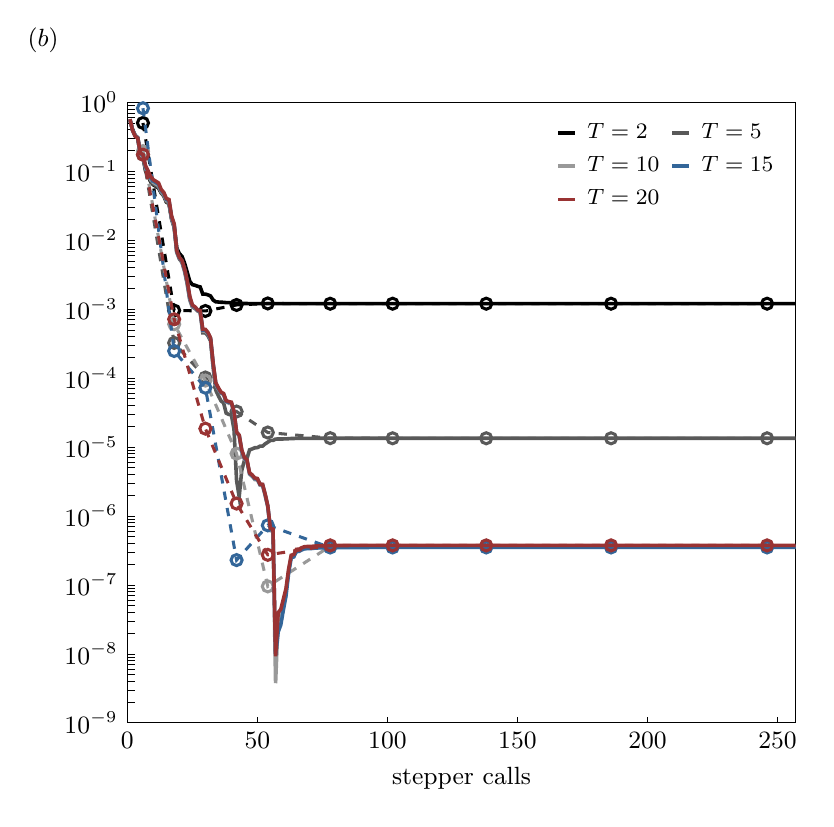
\begin{tikzpicture}

\begin{axis}[%
width=11.252in,
height=7.131in,
at={(1.887in,0.962in)},
scale only axis,
clip=true,
separate axis lines,
every outer x axis line/.append style={black},
every x tick label/.append style={font=\color{black}},
every x tick/.append style={black},
xmin=0,
xmax=257,
xlabel={stepper calls},
every outer y axis line/.append style={black},
every y tick label/.append style={font=\color{black}},
every y tick/.append style={black},
ymode=log,
ymin=1e-09,
ymax=1,
yminorticks=true,
axis background/.style={fill=white},
legend style={legend cell align=left, align=left},
clip=true,
clip mode=individual,
axis lines=box,
xtick pos=bottom,
ytick pos=left,
tick align=inside,
major tick length=2pt,
width=0.7\linewidth,
height=0.65\linewidth,
every axis/.append style={font=\fontsize{9}{9}\selectfont},xlabel style={font=\fontsize{9}{9}\selectfont},title style={font=\fontsize{9}{9}\selectfont},
legend style={font=\fontsize{8}{9}\selectfont,inner sep=1pt,row sep=1pt,column sep=2pt,nodes={scale=1.00},draw=none},legend image post style={xscale=0.35},
legend columns=2,
scaled x ticks=false,
tick label style={/pgf/number format/fixed,/pgf/number format/precision=2},
every x tick label/.append style={font=\fontsize{9}{9}\selectfont\color{black}},
every y tick label/.append style={font=\fontsize{9}{9}\selectfont\color{black}},
,,
colormap={sigmamap}{rgb(0.0000)=(0.0200,0.1880,0.3800); rgb(0.1000)=(0.0743,0.3456,0.5616); rgb(0.2000)=(0.1918,0.4980,0.7060); rgb(0.3000)=(0.3890,0.6708,0.8226); rgb(0.4000)=(0.7552,0.8682,0.9228); rgb(0.5000)=(0.9690,0.9689,0.9689); rgb(0.6000)=(0.9425,0.8044,0.7614); rgb(0.7000)=(0.8767,0.4910,0.4020); rgb(0.8000)=(0.7869,0.2866,0.2470); rgb(0.9000)=(0.6186,0.1239,0.1568); rgb(1.0000)=(0.4040,0.0000,0.1220)}
]
\addplot [color=black, line width=1.3pt]
  table[row sep=crcr]{%
1	0.549669373328673\\
2	0.397017758326252\\
3	0.329385940378878\\
4	0.304042611548967\\
5	0.169444010329133\\
6	0.159452986665028\\
7	0.100626867648435\\
8	0.0849104695143835\\
9	0.0694873979297496\\
10	0.0632602086455798\\
11	0.0602107033749527\\
12	0.0567233098120105\\
13	0.0483275747489066\\
14	0.0438603616932953\\
15	0.0355617152947995\\
16	0.0338823885271802\\
17	0.0205533187125209\\
18	0.0158253009137569\\
19	0.00770254065852706\\
20	0.00636178928833088\\
21	0.00582162810062492\\
22	0.00462227982143794\\
23	0.0034434240593133\\
24	0.00252292974444555\\
25	0.00226168408256191\\
26	0.00221194947129454\\
27	0.0021400268633986\\
28	0.00209449770537478\\
29	0.00164871731744055\\
30	0.00164771495230215\\
31	0.00160538211639674\\
32	0.00154701309238332\\
33	0.00134719680001395\\
34	0.00127497590904898\\
35	0.00126434855840259\\
36	0.00125486412740125\\
37	0.00125208430335636\\
38	0.00123924856778656\\
39	0.00123809692125212\\
40	0.0012377413739315\\
41	0.00122641194599775\\
42	0.00121228121879711\\
43	0.00121099274233937\\
44	0.00120433582689565\\
45	0.00120270089422069\\
46	0.0012021855630201\\
47	0.00119987363566855\\
48	0.00119958893998503\\
49	0.0011992390365001\\
50	0.00119920279807839\\
51	0.00119874912374614\\
52	0.00119871011832831\\
53	0.00119792370841877\\
54	0.00119729006958437\\
55	0.00119658420419771\\
56	0.0011965706750862\\
57	0.001196036488324\\
58	0.00119600588916133\\
59	0.00119599619206095\\
60	0.00119598243518513\\
61	0.00119595528832575\\
62	0.00119588365243689\\
63	0.0011957865724953\\
64	0.00119578007904377\\
65	0.00119573751801717\\
66	0.00119573509137369\\
67	0.00119572086982291\\
68	0.00119570964810775\\
69	0.00119570652683007\\
70	0.00119570638820676\\
71	0.00119570478355878\\
72	0.00119570175073589\\
73	0.00119569979750223\\
74	0.00119569878899582\\
75	0.00119569855114903\\
76	0.00119569690909236\\
77	0.0011956967460316\\
78	0.00119569674115822\\
79	0.00119569636767616\\
80	0.00119569619312675\\
81	0.00119569560737483\\
82	0.0011956955776915\\
83	0.00119569519282965\\
84	0.00119569473647112\\
85	0.00119569467462868\\
86	0.00119569422571662\\
87	0.00119569421020061\\
88	0.00119569419775862\\
89	0.00119569411125754\\
90	0.00119569410667959\\
91	0.00119569410033646\\
92	0.0011956939765608\\
93	0.00119569394254596\\
94	0.0011956939324354\\
95	0.00119569392592682\\
96	0.00119569389279282\\
97	0.00119569389260429\\
98	0.00119569388893417\\
99	0.00119569388694803\\
100	0.00119569388570688\\
101	0.00119569388503786\\
102	0.00119569388456522\\
103	0.00119569388395673\\
104	0.00119569388386028\\
105	0.00119569388317799\\
106	0.00119569388308807\\
107	0.00119569388244497\\
108	0.00119569388203437\\
109	0.0011956938807168\\
110	0.00119569388053328\\
111	0.00119569388050541\\
112	0.00119569388026288\\
113	0.00119569388020301\\
114	0.00119569388019953\\
115	0.00119569388014489\\
116	0.00119569388010265\\
117	0.00119569388006716\\
118	0.00119569388005889\\
119	0.00119569388003516\\
120	0.00119569387999728\\
121	0.00119569387998335\\
122	0.00119569387997921\\
123	0.00119569387995766\\
124	0.00119569387995635\\
125	0.00119569387995265\\
126	0.00119569387995113\\
127	0.0011956938799496\\
128	0.00119569387994046\\
129	0.00119569387993763\\
130	0.00119569387993719\\
131	0.00119569387993632\\
132	0.00119569387993545\\
133	0.00119569387993502\\
134	0.0011956938799348\\
135	0.00119569387993458\\
136	0.00119569387993414\\
137	0.00119569387993414\\
138	0.00119569387993393\\
139	0.00119569387993393\\
140	0.00119569387993393\\
141	0.00119569387993371\\
142	0.00119569387993349\\
143	0.00119569387993349\\
144	0.00119569387993349\\
145	0.00119569387993349\\
146	0.00119569387993349\\
147	0.00119569387993349\\
148	0.00119569387993349\\
149	0.00119569387993349\\
150	0.00119569387993349\\
151	0.00119569387993349\\
152	0.00119569387993349\\
153	0.00119569387993349\\
154	0.00119569387993349\\
155	0.00119569387993349\\
156	0.00119569387993349\\
157	0.00119569387993349\\
158	0.00119569387993349\\
159	0.00119569387993349\\
160	0.00119569387993349\\
161	0.00119569387993349\\
162	0.00119569387993349\\
163	0.00119569387993349\\
164	0.00119569387993349\\
165	0.00119569387993349\\
166	0.00119569387993349\\
167	0.00119569387993349\\
168	0.00119569387993349\\
169	0.00119569387993349\\
170	0.00119569387993349\\
171	0.00119569387993349\\
172	0.00119569387993349\\
173	0.00119569387993349\\
174	0.00119569387993349\\
175	0.00119569387993349\\
176	0.00119569387993349\\
177	0.00119569387993349\\
178	0.00119569387993349\\
179	0.00119569387993349\\
180	0.00119569387993349\\
181	0.00119569387993349\\
182	0.00119569387993349\\
183	0.00119569387993349\\
184	0.00119569387993349\\
185	0.00119569387993349\\
186	0.00119569387993349\\
187	0.00119569387993349\\
188	0.00119569387993349\\
189	0.00119569387993349\\
190	0.00119569387993349\\
191	0.00119569387993349\\
192	0.00119569387993349\\
193	0.00119569387993349\\
194	0.00119569387993349\\
195	0.00119569387993349\\
196	0.00119569387993349\\
197	0.00119569387993349\\
198	0.00119569387993349\\
199	0.00119569387993349\\
200	0.00119569387993349\\
201	0.00119569387993349\\
202	0.00119569387993349\\
203	0.00119569387993349\\
204	0.00119569387993349\\
205	0.00119569387993349\\
206	0.00119569387993349\\
207	0.00119569387993349\\
208	0.00119569387993349\\
209	0.00119569387993349\\
210	0.00119569387993349\\
211	0.00119569387993349\\
212	0.00119569387993349\\
213	0.00119569387993349\\
214	0.00119569387993349\\
215	0.00119569387993349\\
216	0.00119569387993349\\
217	0.00119569387993349\\
218	0.00119569387993349\\
219	0.00119569387993349\\
220	0.00119569387993349\\
221	0.00119569387993349\\
222	0.00119569387993349\\
223	0.00119569387993349\\
224	0.00119569387993349\\
225	0.00119569387993349\\
226	0.00119569387993349\\
227	0.00119569387993349\\
228	0.00119569387993349\\
229	0.00119569387993349\\
230	0.00119569387993349\\
231	0.00119569387993349\\
232	0.00119569387993349\\
233	0.00119569387993349\\
234	0.00119569387993349\\
235	0.00119569387993349\\
236	0.00119569387993349\\
237	0.00119569387993349\\
238	0.00119569387993349\\
239	0.00119569387993349\\
240	0.00119569387993349\\
241	0.00119569387993349\\
242	0.00119569387993349\\
243	0.00119569387993349\\
244	0.00119569387993349\\
245	0.00119569387993349\\
246	0.00119569387993349\\
247	0.00119569387993349\\
248	0.00119569387993349\\
249	0.00119569387993349\\
250	0.00119569387993349\\
251	0.00119569387993349\\
252	0.00119569387993349\\
253	0.00119569387993349\\
254	0.00119569387993349\\
255	0.00119569387993349\\
256	0.00119569387993349\\
257	0.00119569387993349\\
};
\addlegendentry{$T=2$}

\addplot [color=black, dashed, line width=1.1pt, mark size=2.0pt, mark=o, mark options={solid, black}, forget plot]
  table[row sep=crcr]{%
6	0.500186391700627\\
18	0.000953091266489265\\
30	0.000937895531436231\\
42	0.00114613720263973\\
54	0.00120561859610211\\
78	0.00119455605801567\\
102	0.00119526527591131\\
138	0.00119569325590729\\
186	0.00119569419389845\\
246	0.00119569387985054\\
};
\addplot [color=white!35!black, line width=1.3pt]
  table[row sep=crcr]{%
1	0.559033137196902\\
2	0.399370562646894\\
3	0.329302895120021\\
4	0.306698715275885\\
5	0.172052357335026\\
6	0.16319890522921\\
7	0.104969779021928\\
8	0.0883103836569877\\
9	0.0714386473743471\\
10	0.064945741622158\\
11	0.0616826625826992\\
12	0.0580766532695019\\
13	0.0486545368239233\\
14	0.0442166251248846\\
15	0.0358420473896074\\
16	0.0343089376356351\\
17	0.0199915060764878\\
18	0.0151886799857187\\
19	0.006652133182784\\
20	0.00531071631804672\\
21	0.00475147435290793\\
22	0.00352687356420163\\
23	0.0023243251692648\\
24	0.00135701802760233\\
25	0.0010702867649284\\
26	0.00102088761475115\\
27	0.000938600650181147\\
28	0.000901307452132813\\
29	0.000452940546045711\\
30	0.000451819721460005\\
31	0.000409562223026839\\
32	0.000345504828198503\\
33	0.000140740903948513\\
34	6.65259626557667e-05\\
35	5.52609723132258e-05\\
36	4.65584268039886e-05\\
37	4.36867067747377e-05\\
38	3.0892628351158e-05\\
39	2.96437461122934e-05\\
40	2.91802439066835e-05\\
41	1.80562903197952e-05\\
42	3.26595915914533e-06\\
43	1.90065585801823e-06\\
44	4.61522082985248e-06\\
45	6.3331791828639e-06\\
46	6.83399937297337e-06\\
47	9.07655446816112e-06\\
48	9.36127163991361e-06\\
49	9.73366034250314e-06\\
50	9.77047575220323e-06\\
51	1.02653611725188e-05\\
52	1.02994007819449e-05\\
53	1.10935563276389e-05\\
54	1.1718338308664e-05\\
55	1.24309056312515e-05\\
56	1.24456567959361e-05\\
57	1.30120941042536e-05\\
58	1.30420100392807e-05\\
59	1.30511795746009e-05\\
60	1.30657238665149e-05\\
61	1.30916871846514e-05\\
62	1.31658799261434e-05\\
63	1.32659928977106e-05\\
64	1.32723957246663e-05\\
65	1.33173964641523e-05\\
66	1.33196958058559e-05\\
67	1.33339537340158e-05\\
68	1.33450894980249e-05\\
69	1.33480778203941e-05\\
70	1.3348237115529e-05\\
71	1.3349925219261e-05\\
72	1.33531694088253e-05\\
73	1.33550698724182e-05\\
74	1.33560507515186e-05\\
75	1.33562986059396e-05\\
76	1.33579735548693e-05\\
77	1.33581497486299e-05\\
78	1.33581547843016e-05\\
79	1.33585397589709e-05\\
80	1.33587240048085e-05\\
81	1.33593119382798e-05\\
82	1.33593377601764e-05\\
83	1.33597261906152e-05\\
84	1.33601805009195e-05\\
85	1.33602425083795e-05\\
86	1.33607035448835e-05\\
87	1.33607181576611e-05\\
88	1.33607300272703e-05\\
89	1.33608187441448e-05\\
90	1.33608246069358e-05\\
91	1.3360831604489e-05\\
92	1.33609591350746e-05\\
93	1.33609961007948e-05\\
94	1.3361005875671e-05\\
95	1.3361012935255e-05\\
96	1.33610477606609e-05\\
97	1.33610479318107e-05\\
98	1.33610517662945e-05\\
99	1.33610537608238e-05\\
100	1.3361055033209e-05\\
101	1.33610557188127e-05\\
102	1.33610563152629e-05\\
103	1.3361056942854e-05\\
104	1.33610570348957e-05\\
105	1.33610577139699e-05\\
106	1.33610578183173e-05\\
107	1.33610584767982e-05\\
108	1.3361058919427e-05\\
109	1.33610602661487e-05\\
110	1.33610604617843e-05\\
111	1.33610604871492e-05\\
112	1.33610607502151e-05\\
113	1.33610608072231e-05\\
114	1.33610608117436e-05\\
115	1.33610608678727e-05\\
116	1.33610609095614e-05\\
117	1.33610609487388e-05\\
118	1.33610609572774e-05\\
119	1.33610609820144e-05\\
120	1.33610610216941e-05\\
121	1.33610610360089e-05\\
122	1.33610610402782e-05\\
123	1.33610610623782e-05\\
124	1.33610610637595e-05\\
125	1.33610610675266e-05\\
126	1.33610610689078e-05\\
127	1.33610610704146e-05\\
128	1.33610610798323e-05\\
129	1.33610610827203e-05\\
130	1.3361061083097e-05\\
131	1.33610610838504e-05\\
132	1.3361061084855e-05\\
133	1.33610610853573e-05\\
134	1.3361061085734e-05\\
135	1.33610610858595e-05\\
136	1.33610610862362e-05\\
137	1.33610610862362e-05\\
138	1.3361061086613e-05\\
139	1.33610610867385e-05\\
140	1.33610610867385e-05\\
141	1.33610610868641e-05\\
142	1.33610610871152e-05\\
143	1.33610610871152e-05\\
144	1.33610610871152e-05\\
145	1.33610610871152e-05\\
146	1.33610610871152e-05\\
147	1.33610610871152e-05\\
148	1.33610610871152e-05\\
149	1.33610610871152e-05\\
150	1.33610610871152e-05\\
151	1.33610610871152e-05\\
152	1.33610610871152e-05\\
153	1.33610610871152e-05\\
154	1.33610610871152e-05\\
155	1.33610610871152e-05\\
156	1.33610610871152e-05\\
157	1.33610610871152e-05\\
158	1.33610610871152e-05\\
159	1.33610610871152e-05\\
160	1.33610610871152e-05\\
161	1.33610610871152e-05\\
162	1.33610610871152e-05\\
163	1.33610610871152e-05\\
164	1.33610610871152e-05\\
165	1.33610610871152e-05\\
166	1.33610610871152e-05\\
167	1.33610610871152e-05\\
168	1.33610610871152e-05\\
169	1.33610610871152e-05\\
170	1.33610610871152e-05\\
171	1.33610610871152e-05\\
172	1.33610610871152e-05\\
173	1.33610610871152e-05\\
174	1.33610610871152e-05\\
175	1.33610610871152e-05\\
176	1.33610610871152e-05\\
177	1.33610610871152e-05\\
178	1.33610610871152e-05\\
179	1.33610610871152e-05\\
180	1.33610610871152e-05\\
181	1.33610610871152e-05\\
182	1.33610610871152e-05\\
183	1.33610610871152e-05\\
184	1.33610610871152e-05\\
185	1.33610610871152e-05\\
186	1.33610610871152e-05\\
187	1.33610610871152e-05\\
188	1.33610610871152e-05\\
189	1.33610610871152e-05\\
190	1.33610610871152e-05\\
191	1.33610610871152e-05\\
192	1.33610610871152e-05\\
193	1.33610610871152e-05\\
194	1.33610610871152e-05\\
195	1.33610610871152e-05\\
196	1.33610610871152e-05\\
197	1.33610610871152e-05\\
198	1.33610610871152e-05\\
199	1.33610610871152e-05\\
200	1.33610610871152e-05\\
201	1.33610610871152e-05\\
202	1.33610610871152e-05\\
203	1.33610610871152e-05\\
204	1.33610610871152e-05\\
205	1.33610610871152e-05\\
206	1.33610610871152e-05\\
207	1.33610610871152e-05\\
208	1.33610610871152e-05\\
209	1.33610610871152e-05\\
210	1.33610610871152e-05\\
211	1.33610610871152e-05\\
212	1.33610610871152e-05\\
213	1.33610610871152e-05\\
214	1.33610610871152e-05\\
215	1.33610610871152e-05\\
216	1.33610610871152e-05\\
217	1.33610610871152e-05\\
218	1.33610610871152e-05\\
219	1.33610610871152e-05\\
220	1.33610610871152e-05\\
221	1.33610610871152e-05\\
222	1.33610610871152e-05\\
223	1.33610610871152e-05\\
224	1.33610610871152e-05\\
225	1.33610610871152e-05\\
226	1.33610610871152e-05\\
227	1.33610610871152e-05\\
228	1.33610610871152e-05\\
229	1.33610610871152e-05\\
230	1.33610610871152e-05\\
231	1.33610610871152e-05\\
232	1.33610610871152e-05\\
233	1.33610610871152e-05\\
234	1.33610610871152e-05\\
235	1.33610610871152e-05\\
236	1.33610610871152e-05\\
237	1.33610610871152e-05\\
238	1.33610610871152e-05\\
239	1.33610610871152e-05\\
240	1.33610610871152e-05\\
241	1.33610610871152e-05\\
242	1.33610610871152e-05\\
243	1.33610610871152e-05\\
244	1.33610610871152e-05\\
245	1.33610610871152e-05\\
246	1.33610610871152e-05\\
247	1.33610610871152e-05\\
248	1.33610610871152e-05\\
249	1.33610610871152e-05\\
250	1.33610610871152e-05\\
251	1.33610610871152e-05\\
252	1.33610610871152e-05\\
253	1.33610610871152e-05\\
254	1.33610610871152e-05\\
255	1.33610610871152e-05\\
256	1.33610610871152e-05\\
257	1.33610610871152e-05\\
};
\addlegendentry{$T=5$}

\addplot [color=white!35!black, dashed, line width=1.1pt, mark size=2.0pt, mark=o, mark options={solid, white!35!black}, forget plot]
  table[row sep=crcr]{%
6	0.173444432589479\\
18	0.000322957642254964\\
30	0.000101687665819906\\
42	3.26495648006814e-05\\
54	1.62064647237235e-05\\
78	1.34198389411002e-05\\
102	1.33590527996498e-05\\
138	1.33610355388322e-05\\
186	1.33610611655955e-05\\
246	1.33610610878686e-05\\
};
\addplot [color=white!60!black, line width=1.3pt]
  table[row sep=crcr]{%
1	0.564607223850406\\
2	0.396758973927432\\
3	0.326445192001137\\
4	0.305342094296728\\
5	0.175675676464535\\
6	0.167903493405876\\
7	0.110982018363616\\
8	0.0932041795791994\\
9	0.0756335859496363\\
10	0.0686612058289143\\
11	0.0651210578167606\\
12	0.0614886904025271\\
13	0.0506130701614662\\
14	0.0460435679071081\\
15	0.037521905756448\\
16	0.0361065407031926\\
17	0.0207935070318107\\
18	0.0159310964064198\\
19	0.00680931860605786\\
20	0.00545037290468793\\
21	0.00488304372519022\\
22	0.00365450952483655\\
23	0.00243521282985079\\
24	0.00142129122639922\\
25	0.00109879304218316\\
26	0.00104552799072529\\
27	0.00095420262223343\\
28	0.000924545529589524\\
29	0.00048125790828469\\
30	0.000480294696618071\\
31	0.000435649338525187\\
32	0.000366380621243458\\
33	0.000156105502138586\\
34	8.08270566108681e-05\\
35	6.87871673626111e-05\\
36	6.03888192089379e-05\\
37	5.74653367814186e-05\\
38	4.47684286374736e-05\\
39	4.34636625254548e-05\\
40	4.28406773344513e-05\\
41	3.17612705488361e-05\\
42	1.61629785633702e-05\\
43	1.47061215135406e-05\\
44	8.51261199210358e-06\\
45	6.705935367087e-06\\
46	6.20142788109269e-06\\
47	4.02058535815122e-06\\
48	3.74431287273559e-06\\
49	3.36537183448011e-06\\
50	3.32277108203417e-06\\
51	2.7887766861761e-06\\
52	2.75716296231618e-06\\
53	1.96254667866241e-06\\
54	1.33676872918941e-06\\
55	6.11941895989095e-07\\
56	5.9727412945619e-07\\
57	3.75051588558086e-09\\
58	3.36021656519237e-08\\
59	4.06455718167724e-08\\
60	5.6610641453684e-08\\
61	8.17774088124832e-08\\
62	1.57907492776768e-07\\
63	2.58974101885202e-07\\
64	2.65489923131242e-07\\
65	3.12904836386055e-07\\
66	3.14957046412481e-07\\
67	3.29406420299031e-07\\
68	3.4055024922441e-07\\
69	3.4355238615584e-07\\
70	3.43735687345281e-07\\
71	3.45522129333168e-07\\
72	3.48967645564236e-07\\
73	3.50819817227821e-07\\
74	3.51798462951844e-07\\
75	3.52044614345287e-07\\
76	3.53761955151238e-07\\
77	3.53945461897642e-07\\
78	3.53951140478496e-07\\
79	3.54327414265969e-07\\
80	3.54516676793354e-07\\
81	3.55105940892562e-07\\
82	3.5512811593124e-07\\
83	3.55534876327613e-07\\
84	3.559866825326e-07\\
85	3.56048693766554e-07\\
86	3.56531969905423e-07\\
87	3.56544973569101e-07\\
88	3.56557102546048e-07\\
89	3.56649536396507e-07\\
90	3.56657281894477e-07\\
91	3.56665061992985e-07\\
92	3.5679827257809e-07\\
93	3.56837899495915e-07\\
94	3.56847596203823e-07\\
95	3.56854907334817e-07\\
96	3.56891937910082e-07\\
97	3.56892115005312e-07\\
98	3.56896002543236e-07\\
99	3.56897989655884e-07\\
100	3.56899258342296e-07\\
101	3.56899965235019e-07\\
102	3.56900740398696e-07\\
103	3.56901402273514e-07\\
104	3.5690149509969e-07\\
105	3.5690220106229e-07\\
106	3.56902322536224e-07\\
107	3.56902971761382e-07\\
108	3.56903453936628e-07\\
109	3.56904865303756e-07\\
110	3.56905078487719e-07\\
111	3.56905100810647e-07\\
112	3.56905379289175e-07\\
113	3.56905435840593e-07\\
114	3.56905442165422e-07\\
115	3.56905498530816e-07\\
116	3.56905540200282e-07\\
117	3.56905582985894e-07\\
118	3.56905592287114e-07\\
119	3.56905617400408e-07\\
120	3.5690566018602e-07\\
121	3.56905675440021e-07\\
122	3.56905679904606e-07\\
123	3.56905703343681e-07\\
124	3.569057050179e-07\\
125	3.56905708738389e-07\\
126	3.56905710226584e-07\\
127	3.56905711900803e-07\\
128	3.56905721946121e-07\\
129	3.56905724922511e-07\\
130	3.5690572529456e-07\\
131	3.56905726038658e-07\\
132	3.5690572696878e-07\\
133	3.56905727526853e-07\\
134	3.56905727898902e-07\\
135	3.56905728084926e-07\\
136	3.56905728642999e-07\\
137	3.56905728642999e-07\\
138	3.56905729015048e-07\\
139	3.56905729201073e-07\\
140	3.56905729201073e-07\\
141	3.56905729387097e-07\\
142	3.56905729759146e-07\\
143	3.56905729759146e-07\\
144	3.56905729759146e-07\\
145	3.56905729759146e-07\\
146	3.56905729759146e-07\\
147	3.56905729759146e-07\\
148	3.56905729759146e-07\\
149	3.56905729759146e-07\\
150	3.56905729759146e-07\\
151	3.56905729759146e-07\\
152	3.56905729759146e-07\\
153	3.56905729759146e-07\\
154	3.56905729759146e-07\\
155	3.56905729759146e-07\\
156	3.56905729759146e-07\\
157	3.56905729759146e-07\\
158	3.56905729759146e-07\\
159	3.56905729759146e-07\\
160	3.56905729759146e-07\\
161	3.56905729759146e-07\\
162	3.56905729759146e-07\\
163	3.56905729759146e-07\\
164	3.56905729759146e-07\\
165	3.56905729759146e-07\\
166	3.56905729759146e-07\\
167	3.56905729759146e-07\\
168	3.56905729759146e-07\\
169	3.56905729759146e-07\\
170	3.56905729759146e-07\\
171	3.56905729759146e-07\\
172	3.56905729759146e-07\\
173	3.56905729759146e-07\\
174	3.56905729759146e-07\\
175	3.56905729759146e-07\\
176	3.56905729759146e-07\\
177	3.56905729759146e-07\\
178	3.56905729759146e-07\\
179	3.56905729759146e-07\\
180	3.56905729759146e-07\\
181	3.56905729759146e-07\\
182	3.56905729759146e-07\\
183	3.56905729759146e-07\\
184	3.56905729759146e-07\\
185	3.56905729759146e-07\\
186	3.56905729759146e-07\\
187	3.56905729759146e-07\\
188	3.56905729759146e-07\\
189	3.56905729759146e-07\\
190	3.56905729759146e-07\\
191	3.56905729759146e-07\\
192	3.56905729759146e-07\\
193	3.56905729759146e-07\\
194	3.56905729759146e-07\\
195	3.56905729759146e-07\\
196	3.56905729759146e-07\\
197	3.56905729759146e-07\\
198	3.56905729759146e-07\\
199	3.56905729759146e-07\\
200	3.56905729759146e-07\\
201	3.56905729759146e-07\\
202	3.56905729759146e-07\\
203	3.56905729759146e-07\\
204	3.56905729759146e-07\\
205	3.56905729759146e-07\\
206	3.56905729759146e-07\\
207	3.56905729759146e-07\\
208	3.56905729759146e-07\\
209	3.56905729759146e-07\\
210	3.56905729759146e-07\\
211	3.56905729759146e-07\\
212	3.56905729759146e-07\\
213	3.56905729759146e-07\\
214	3.56905729759146e-07\\
215	3.56905729759146e-07\\
216	3.56905729759146e-07\\
217	3.56905729759146e-07\\
218	3.56905729759146e-07\\
219	3.56905729759146e-07\\
220	3.56905729759146e-07\\
221	3.56905729759146e-07\\
222	3.56905729759146e-07\\
223	3.56905729759146e-07\\
224	3.56905729759146e-07\\
225	3.56905729759146e-07\\
226	3.56905729759146e-07\\
227	3.56905729759146e-07\\
228	3.56905729759146e-07\\
229	3.56905729759146e-07\\
230	3.56905729759146e-07\\
231	3.56905729759146e-07\\
232	3.56905729759146e-07\\
233	3.56905729759146e-07\\
234	3.56905729759146e-07\\
235	3.56905729759146e-07\\
236	3.56905729759146e-07\\
237	3.56905729759146e-07\\
238	3.56905729759146e-07\\
239	3.56905729759146e-07\\
240	3.56905729759146e-07\\
241	3.56905729759146e-07\\
242	3.56905729759146e-07\\
243	3.56905729759146e-07\\
244	3.56905729759146e-07\\
245	3.56905729759146e-07\\
246	3.56905729759146e-07\\
247	3.56905729759146e-07\\
248	3.56905729759146e-07\\
249	3.56905729759146e-07\\
250	3.56905729759146e-07\\
251	3.56905729759146e-07\\
252	3.56905729759146e-07\\
253	3.56905729759146e-07\\
254	3.56905729759146e-07\\
255	3.56905729759146e-07\\
256	3.56905729759146e-07\\
257	3.56905729759146e-07\\
};
\addlegendentry{$T=10$}

\addplot [color=white!60!black, dashed, line width=1.1pt, mark size=2.0pt, mark=o, mark options={solid, white!60!black}, forget plot]
  table[row sep=crcr]{%
6	0.195015805283674\\
18	0.000603102194024149\\
30	9.17721279357794e-05\\
42	8.00760381008745e-06\\
54	9.51141711308382e-08\\
78	3.62838592575086e-07\\
102	3.5667661094585e-07\\
138	3.56905727898902e-07\\
186	3.56905730503243e-07\\
246	3.56905728642999e-07\\
};
\addplot [color=mycolor1, line width=1.3pt]
  table[row sep=crcr]{%
1	0.566656855065321\\
2	0.392875725684473\\
3	0.323772573360371\\
4	0.302801358166162\\
5	0.178595981845843\\
6	0.171587776627804\\
7	0.115791401523224\\
8	0.0970557094110618\\
9	0.0793371199946198\\
10	0.0720374269239434\\
11	0.068266173476437\\
12	0.0646073113866519\\
13	0.0525013358978267\\
14	0.0476953080114036\\
15	0.0389164095610798\\
16	0.0375455584116823\\
17	0.0215399832699583\\
18	0.0166151049257236\\
19	0.00692206348940702\\
20	0.00553674357961893\\
21	0.00498166842603597\\
22	0.00374896230271129\\
23	0.00252717681739777\\
24	0.0014743491939089\\
25	0.00111860408408585\\
26	0.00105951972411547\\
27	0.000962173331887127\\
28	0.000935217272346847\\
29	0.000495319031786381\\
30	0.000494466321345801\\
31	0.000446720213088636\\
32	0.000373533603640214\\
33	0.000159348556174509\\
34	8.29398214375151e-05\\
35	7.03619109225198e-05\\
36	6.14446590014436e-05\\
37	5.85079068285983e-05\\
38	4.57862100247197e-05\\
39	4.447638060846e-05\\
40	4.37008017074584e-05\\
41	3.24589285546669e-05\\
42	1.6238922261738e-05\\
43	1.47273643345182e-05\\
44	8.76789612878521e-06\\
45	6.86466479015716e-06\\
46	6.34077289656015e-06\\
47	4.12495145987292e-06\\
48	3.85312104754706e-06\\
49	3.47330018353092e-06\\
50	3.4223196416228e-06\\
51	2.85874500519026e-06\\
52	2.82707558876772e-06\\
53	2.03010681674796e-06\\
54	1.3888612900811e-06\\
55	6.51362104441099e-07\\
56	6.3723823857289e-07\\
57	9.35149208097676e-09\\
58	2.07968674990126e-08\\
59	2.6304002017418e-08\\
60	4.34915151341377e-08\\
61	6.88666338902863e-08\\
62	1.46862583115573e-07\\
63	2.47544103202229e-07\\
64	2.54297800845049e-07\\
65	3.04049677345911e-07\\
66	3.05923451899042e-07\\
67	3.20680472215724e-07\\
68	3.32149361028681e-07\\
69	3.35185165238863e-07\\
70	3.35393106301297e-07\\
71	3.37285369297977e-07\\
72	3.40859442088952e-07\\
73	3.42710173612424e-07\\
74	3.43707257990091e-07\\
75	3.43949065854969e-07\\
76	3.45736820472359e-07\\
77	3.45921035283644e-07\\
78	3.45927147681899e-07\\
79	3.4628508272022e-07\\
80	3.46482007633499e-07\\
81	3.47078208696351e-07\\
82	3.47098781888717e-07\\
83	3.4752664288393e-07\\
84	3.47983009323369e-07\\
85	3.48045073364963e-07\\
86	3.48551242790067e-07\\
87	3.4856277244648e-07\\
88	3.48575653269912e-07\\
89	3.48672074959069e-07\\
90	3.48681387586927e-07\\
91	3.48689709795425e-07\\
92	3.48828301862211e-07\\
93	3.48869767027683e-07\\
94	3.48879543977565e-07\\
95	3.48886811976983e-07\\
96	3.48925617111071e-07\\
97	3.48925820734577e-07\\
98	3.48929660372203e-07\\
99	3.48931645911217e-07\\
100	3.48932940003223e-07\\
101	3.4893364957994e-07\\
102	3.48934588463919e-07\\
103	3.48935290318722e-07\\
104	3.4893539288588e-07\\
105	3.48936144765254e-07\\
106	3.48936276709257e-07\\
107	3.48936909738308e-07\\
108	3.48937422238359e-07\\
109	3.48938898466807e-07\\
110	3.48939126934731e-07\\
111	3.48939147582456e-07\\
112	3.48939432621791e-07\\
113	3.4893949003254e-07\\
114	3.48939498090189e-07\\
115	3.48939554493732e-07\\
116	3.48939596460654e-07\\
117	3.4893964178493e-07\\
118	3.48939651856991e-07\\
119	3.4893967737288e-07\\
120	3.48939723704361e-07\\
121	3.48939739987527e-07\\
122	3.48939744519955e-07\\
123	3.48939769700108e-07\\
124	3.48939771546653e-07\\
125	3.48939775071874e-07\\
126	3.48939776582683e-07\\
127	3.48939778429228e-07\\
128	3.48939789004892e-07\\
129	3.4893979202651e-07\\
130	3.48939792530114e-07\\
131	3.48939793201584e-07\\
132	3.4893979420879e-07\\
133	3.48939794712394e-07\\
134	3.48939795215997e-07\\
135	3.48939795383864e-07\\
136	3.48939795887467e-07\\
137	3.48939795887467e-07\\
138	3.48939796223203e-07\\
139	3.4893979639107e-07\\
140	3.4893979639107e-07\\
141	3.48939796558938e-07\\
142	3.48939796894673e-07\\
143	3.48939796894673e-07\\
144	3.48939796894673e-07\\
145	3.48939796894673e-07\\
146	3.48939796894673e-07\\
147	3.48939796894673e-07\\
148	3.48939796894673e-07\\
149	3.48939796894673e-07\\
150	3.48939796894673e-07\\
151	3.48939796894673e-07\\
152	3.48939796894673e-07\\
153	3.48939796894673e-07\\
154	3.48939796894673e-07\\
155	3.48939796894673e-07\\
156	3.48939796894673e-07\\
157	3.48939796894673e-07\\
158	3.48939796894673e-07\\
159	3.48939796894673e-07\\
160	3.48939796894673e-07\\
161	3.48939796894673e-07\\
162	3.48939796894673e-07\\
163	3.48939796894673e-07\\
164	3.48939796894673e-07\\
165	3.48939796894673e-07\\
166	3.48939796894673e-07\\
167	3.48939796894673e-07\\
168	3.48939796894673e-07\\
169	3.48939796894673e-07\\
170	3.48939796894673e-07\\
171	3.48939796894673e-07\\
172	3.48939796894673e-07\\
173	3.48939796894673e-07\\
174	3.48939796894673e-07\\
175	3.48939796894673e-07\\
176	3.48939796894673e-07\\
177	3.48939796894673e-07\\
178	3.48939796894673e-07\\
179	3.48939796894673e-07\\
180	3.48939796894673e-07\\
181	3.48939796894673e-07\\
182	3.48939796894673e-07\\
183	3.48939796894673e-07\\
184	3.48939796894673e-07\\
185	3.48939796894673e-07\\
186	3.48939796894673e-07\\
187	3.48939796894673e-07\\
188	3.48939796894673e-07\\
189	3.48939796894673e-07\\
190	3.48939796894673e-07\\
191	3.48939796894673e-07\\
192	3.48939796894673e-07\\
193	3.48939796894673e-07\\
194	3.48939796894673e-07\\
195	3.48939796894673e-07\\
196	3.48939796894673e-07\\
197	3.48939796894673e-07\\
198	3.48939796894673e-07\\
199	3.48939796894673e-07\\
200	3.48939796894673e-07\\
201	3.48939796894673e-07\\
202	3.48939796894673e-07\\
203	3.48939796894673e-07\\
204	3.48939796894673e-07\\
205	3.48939796894673e-07\\
206	3.48939796894673e-07\\
207	3.48939796894673e-07\\
208	3.48939796894673e-07\\
209	3.48939796894673e-07\\
210	3.48939796894673e-07\\
211	3.48939796894673e-07\\
212	3.48939796894673e-07\\
213	3.48939796894673e-07\\
214	3.48939796894673e-07\\
215	3.48939796894673e-07\\
216	3.48939796894673e-07\\
217	3.48939796894673e-07\\
218	3.48939796894673e-07\\
219	3.48939796894673e-07\\
220	3.48939796894673e-07\\
221	3.48939796894673e-07\\
222	3.48939796894673e-07\\
223	3.48939796894673e-07\\
224	3.48939796894673e-07\\
225	3.48939796894673e-07\\
226	3.48939796894673e-07\\
227	3.48939796894673e-07\\
228	3.48939796894673e-07\\
229	3.48939796894673e-07\\
230	3.48939796894673e-07\\
231	3.48939796894673e-07\\
232	3.48939796894673e-07\\
233	3.48939796894673e-07\\
234	3.48939796894673e-07\\
235	3.48939796894673e-07\\
236	3.48939796894673e-07\\
237	3.48939796894673e-07\\
238	3.48939796894673e-07\\
239	3.48939796894673e-07\\
240	3.48939796894673e-07\\
241	3.48939796894673e-07\\
242	3.48939796894673e-07\\
243	3.48939796894673e-07\\
244	3.48939796894673e-07\\
245	3.48939796894673e-07\\
246	3.48939796894673e-07\\
247	3.48939796894673e-07\\
248	3.48939796894673e-07\\
249	3.48939796894673e-07\\
250	3.48939796894673e-07\\
251	3.48939796894673e-07\\
252	3.48939796894673e-07\\
253	3.48939796894673e-07\\
254	3.48939796894673e-07\\
255	3.48939796894673e-07\\
256	3.48939796894673e-07\\
257	3.48939796894673e-07\\
};
\addlegendentry{$T=15$}

\addplot [color=mycolor1, dashed, line width=1.1pt, mark size=2.0pt, mark=o, mark options={solid, mycolor1}, forget plot]
  table[row sep=crcr]{%
6	0.816868180679755\\
18	0.000246780445434153\\
30	7.22780370615801e-05\\
42	2.28708801699798e-07\\
54	7.29981302074725e-07\\
78	3.48475742115126e-07\\
102	3.48938569614007e-07\\
138	3.48939797734012e-07\\
186	3.48939797566144e-07\\
246	3.48939797734012e-07\\
};
\addplot [color=red!60!teal, line width=1.3pt]
  table[row sep=crcr]{%
1	0.567622633937709\\
2	0.389053383852605\\
3	0.321379058864112\\
4	0.300316175834723\\
5	0.180989383558685\\
6	0.174641644194835\\
7	0.119806200761475\\
8	0.100235228438087\\
9	0.0826144240859506\\
10	0.0750849512158574\\
11	0.0711210713964446\\
12	0.0674137274725377\\
13	0.0542517024716162\\
14	0.049188870992894\\
15	0.0401385995807562\\
16	0.0387922841897729\\
17	0.0222609311499474\\
18	0.0172654941549523\\
19	0.00701838794087909\\
20	0.0056097896523553\\
21	0.00507751122920044\\
22	0.00384084280965212\\
23	0.00261957051818231\\
24	0.00152989766845017\\
25	0.00114214985799079\\
26	0.00107701695694854\\
27	0.000974432491025389\\
28	0.000948067991377848\\
29	0.000508745144464383\\
30	0.000507844931534173\\
31	0.000457011942330344\\
32	0.000380240768015184\\
33	0.000163041080796977\\
34	8.52805210804461e-05\\
35	7.22625095956086e-05\\
36	6.2515093026299e-05\\
37	5.95940461329791e-05\\
38	4.68084354259516e-05\\
39	4.55132877191635e-05\\
40	4.45843247689138e-05\\
41	3.31125370677244e-05\\
42	1.64057710327918e-05\\
43	1.48576497539357e-05\\
44	9.05703472463093e-06\\
45	7.05210037598223e-06\\
46	6.5058243837547e-06\\
47	4.20478891782225e-06\\
48	3.93309372534775e-06\\
49	3.55174526691527e-06\\
50	3.49121351060755e-06\\
51	2.90251236554197e-06\\
52	2.87014115404481e-06\\
53	2.06793938504974e-06\\
54	1.40593602753245e-06\\
55	6.56133632421202e-07\\
56	6.42770920735969e-07\\
57	9.19148907733855e-09\\
58	3.96513874145718e-08\\
59	4.42471699258408e-08\\
60	6.24698826862706e-08\\
61	8.85539850274795e-08\\
62	1.68571700956209e-07\\
63	2.68717910376782e-07\\
64	2.75724281197083e-07\\
65	3.27675940855192e-07\\
66	3.29446927821112e-07\\
67	3.44628179249239e-07\\
68	3.56605889577629e-07\\
69	3.59650027244835e-07\\
70	3.59880755931486e-07\\
71	3.61887419756041e-07\\
72	3.65570686960882e-07\\
73	3.67442175664221e-07\\
74	3.68473529888335e-07\\
75	3.68710653128182e-07\\
76	3.70582486681397e-07\\
77	3.70762192254e-07\\
78	3.70768556657279e-07\\
79	3.71106412566622e-07\\
80	3.71314071187735e-07\\
81	3.71920821994808e-07\\
82	3.71940689650113e-07\\
83	3.72388485036143e-07\\
84	3.72853409324095e-07\\
85	3.72915780378445e-07\\
86	3.73443103589051e-07\\
87	3.73453309417857e-07\\
88	3.73467174142956e-07\\
89	3.7356758412684e-07\\
90	3.73578139694698e-07\\
91	3.73586855302681e-07\\
92	3.73730472563973e-07\\
93	3.73773415173991e-07\\
94	3.73783264907817e-07\\
95	3.73790367250716e-07\\
96	3.73830595390258e-07\\
97	3.73830837241494e-07\\
98	3.73834585772679e-07\\
99	3.73836580882403e-07\\
100	3.73837928665234e-07\\
101	3.73838632706567e-07\\
102	3.73839719570376e-07\\
103	3.73840462073227e-07\\
104	3.7384057941345e-07\\
105	3.73841381564247e-07\\
106	3.73841519439008e-07\\
107	3.73842137756791e-07\\
108	3.73842674262363e-07\\
109	3.73844207507934e-07\\
110	3.73844448218362e-07\\
111	3.73844467938038e-07\\
112	3.73844756888336e-07\\
113	3.73844815069529e-07\\
114	3.73844825173826e-07\\
115	3.73844881562322e-07\\
116	3.73844923772207e-07\\
117	3.73844971034241e-07\\
118	3.73844981953401e-07\\
119	3.73845008029006e-07\\
120	3.73845057572655e-07\\
121	3.73845074684771e-07\\
122	3.73845079410974e-07\\
123	3.73845106627387e-07\\
124	3.73845108583057e-07\\
125	3.73845112168453e-07\\
126	3.73845113635206e-07\\
127	3.73845115590876e-07\\
128	3.73845126510036e-07\\
129	3.73845129606514e-07\\
130	3.73845130095432e-07\\
131	3.73845130910294e-07\\
132	3.73845132051102e-07\\
133	3.73845132702992e-07\\
134	3.7384513319191e-07\\
135	3.73845133354882e-07\\
136	3.738451338438e-07\\
137	3.738451338438e-07\\
138	3.73845134169745e-07\\
139	3.73845134332717e-07\\
140	3.73845134332717e-07\\
141	3.7384513449569e-07\\
142	3.73845134821635e-07\\
143	3.73845134821635e-07\\
144	3.73845134821635e-07\\
145	3.73845134821635e-07\\
146	3.73845134821635e-07\\
147	3.73845134821635e-07\\
148	3.73845134821635e-07\\
149	3.73845134821635e-07\\
150	3.73845134821635e-07\\
151	3.73845134821635e-07\\
152	3.73845134821635e-07\\
153	3.73845134821635e-07\\
154	3.73845134821635e-07\\
155	3.73845134821635e-07\\
156	3.73845134821635e-07\\
157	3.73845134821635e-07\\
158	3.73845134821635e-07\\
159	3.73845134821635e-07\\
160	3.73845134821635e-07\\
161	3.73845134821635e-07\\
162	3.73845134821635e-07\\
163	3.73845134821635e-07\\
164	3.73845134821635e-07\\
165	3.73845134821635e-07\\
166	3.73845134821635e-07\\
167	3.73845134821635e-07\\
168	3.73845134821635e-07\\
169	3.73845134821635e-07\\
170	3.73845134821635e-07\\
171	3.73845134821635e-07\\
172	3.73845134821635e-07\\
173	3.73845134821635e-07\\
174	3.73845134821635e-07\\
175	3.73845134821635e-07\\
176	3.73845134821635e-07\\
177	3.73845134821635e-07\\
178	3.73845134821635e-07\\
179	3.73845134821635e-07\\
180	3.73845134821635e-07\\
181	3.73845134821635e-07\\
182	3.73845134821635e-07\\
183	3.73845134821635e-07\\
184	3.73845134821635e-07\\
185	3.73845134821635e-07\\
186	3.73845134821635e-07\\
187	3.73845134821635e-07\\
188	3.73845134821635e-07\\
189	3.73845134821635e-07\\
190	3.73845134821635e-07\\
191	3.73845134821635e-07\\
192	3.73845134821635e-07\\
193	3.73845134821635e-07\\
194	3.73845134821635e-07\\
195	3.73845134821635e-07\\
196	3.73845134821635e-07\\
197	3.73845134821635e-07\\
198	3.73845134821635e-07\\
199	3.73845134821635e-07\\
200	3.73845134821635e-07\\
201	3.73845134821635e-07\\
202	3.73845134821635e-07\\
203	3.73845134821635e-07\\
204	3.73845134821635e-07\\
205	3.73845134821635e-07\\
206	3.73845134821635e-07\\
207	3.73845134821635e-07\\
208	3.73845134821635e-07\\
209	3.73845134821635e-07\\
210	3.73845134821635e-07\\
211	3.73845134821635e-07\\
212	3.73845134821635e-07\\
213	3.73845134821635e-07\\
214	3.73845134821635e-07\\
215	3.73845134821635e-07\\
216	3.73845134821635e-07\\
217	3.73845134821635e-07\\
218	3.73845134821635e-07\\
219	3.73845134821635e-07\\
220	3.73845134821635e-07\\
221	3.73845134821635e-07\\
222	3.73845134821635e-07\\
223	3.73845134821635e-07\\
224	3.73845134821635e-07\\
225	3.73845134821635e-07\\
226	3.73845134821635e-07\\
227	3.73845134821635e-07\\
228	3.73845134821635e-07\\
229	3.73845134821635e-07\\
230	3.73845134821635e-07\\
231	3.73845134821635e-07\\
232	3.73845134821635e-07\\
233	3.73845134821635e-07\\
234	3.73845134821635e-07\\
235	3.73845134821635e-07\\
236	3.73845134821635e-07\\
237	3.73845134821635e-07\\
238	3.73845134821635e-07\\
239	3.73845134821635e-07\\
240	3.73845134821635e-07\\
241	3.73845134821635e-07\\
242	3.73845134821635e-07\\
243	3.73845134821635e-07\\
244	3.73845134821635e-07\\
245	3.73845134821635e-07\\
246	3.73845134821635e-07\\
247	3.73845134821635e-07\\
248	3.73845134821635e-07\\
249	3.73845134821635e-07\\
250	3.73845134821635e-07\\
251	3.73845134821635e-07\\
252	3.73845134821635e-07\\
253	3.73845134821635e-07\\
254	3.73845134821635e-07\\
255	3.73845134821635e-07\\
256	3.73845134821635e-07\\
257	3.73845134821635e-07\\
};
\addlegendentry{$T=20$}

\addplot [color=red!60!teal, dashed, line width=1.1pt, mark size=2.0pt, mark=o, mark options={solid, red!60!teal}, forget plot]
  table[row sep=crcr]{%
6	0.173764830829518\\
18	0.000712138773012073\\
30	1.84486100969018e-05\\
42	1.5095497681292e-06\\
54	2.72572906789643e-07\\
78	3.73748170728945e-07\\
102	3.73845113146288e-07\\
138	3.7384513579947e-07\\
186	3.73845136614333e-07\\
246	3.73845136940278e-07\\
};
\node[right, align=left, inner sep=0]
at (rel axis cs:-0.15,1.1) {$(b)$};
\end{axis}
\end{tikzpicture}%
    \end{minipage}
    \caption{Plane-Poiseuille relative error versus stepper calls for \((a)\) slow and \((b)\) fast covariance-spectrum decay. (\solidlegend) deterministic truncation; (\dashlegend\circlegend) SSTE; dotted line: \(\epsilon_{\mathrm{rel}}=10^{-2}\).}
    \label{fig:Poiseuille_eig_vs_sste}
\end{figure}
To demonstrate that the proposed framework applies to fluid-dynamical systems of practical relevance, we next consider plane Poiseuille flow. Plane Poiseuille flow is the steady laminar flow between two plates separated by a distance \(2h\) in the wall-normal direction. The flow is directed along the streamwise coordinate \(x\), while the plates are taken to be infinite in both the streamwise and spanwise directions. It is driven by a constant pressure gradient, and the base-flow velocity profile is
\begin{equation}
  U(y) = -\frac{1}{2\mu}\frac{dp}{dx}\left(h^2-y^2\right).
\end{equation}
The flow is non-dimensionalized using the channel half-height and the centerline velocity.

Because the governing equations and the base flow are homogeneous in the streamwise and spanwise directions, it is convenient to represent perturbations in Fourier space with respect to \(x\) and \(z\), as in \citet{schmid-henningson-2001}. The associated streamwise and spanwise wavenumbers are denoted here by \(k_x\) and \(k_z\), respectively. For example, the transformed wall-normal velocity may be written as
\begin{equation}
  \hat{v}(y,k_x,k_z)
  =
  \int_{-\infty}^{\infty}
  \int_{-\infty}^{\infty}
  v(x,y,z)\,
  \exp\!\left[-i(k_x x+k_z z)\right]
  \,dx\,dz.
\end{equation}
Employing the standard velocity-vorticity formulation of the linearized Navier--Stokes equations yields the Orr--Sommerfeld/Squire system for the perturbation dynamics, following \citet{schmid-henningson-2001},
\begin{equation}
  \frac{\partial}{\partial t}
  \begin{bmatrix}
    \hat{v}\\
    \hat{\eta}
  \end{bmatrix}
  =
  -i
  \begin{bmatrix}
    \mathcal{L}_{OS} & 0\\
    \mathcal{L}_{C} & \mathcal{L}_{SQ}
  \end{bmatrix}
  \begin{bmatrix}
    \hat{v}\\
    \hat{\eta}
  \end{bmatrix},
\end{equation}
where \(\hat{\eta}\) denotes the transformed wall-normal vorticity and
\begin{equation}
  k^2 = k_x^2 + k_z^2.
\end{equation}
The Orr--Sommerfeld, coupling, and Squire operators are
\begin{align}
  \mathcal{L}_{OS}
  &=
  -\left(
    \frac{\partial^2}{\partial y^2}-k^2
  \right)^{-1}
  \left[
    \frac{1}{i\Rey}
    \left(
      \frac{\partial^2}{\partial y^2}-k^2
    \right)^2
    - k_x U
    \left(
      \frac{\partial^2}{\partial y^2}-k^2
    \right)
    + k_x U''
  \right], \\
  \mathcal{L}_{C}
  &= k_z U'', \\
  \mathcal{L}_{SQ}
  &= k_x U - \frac{1}{i\Rey}
  \left(
    \frac{\partial^2}{\partial y^2}-k^2
  \right).
\end{align}
All quantities are non-dimensional, \(U=U(y)\) denotes the base flow, and \((\cdot)'\) indicates differentiation with respect to \(y\). The disturbance energy in the transformed velocity-vorticity variables is then given, in the standard formulation of \citet{schmid-henningson-2001}, by
\begin{equation}
  e
  =
  \frac{1}{4\pi^2}
  \int_{-\infty}^{\infty}
  \int_{-\infty}^{\infty}
  \frac{1}{2k^2}
  \int_{-1}^{1}
  \left(
    \left|\frac{\partial \hat{v}}{\partial y}\right|^2
    +
    k^2 |\hat{v}|^2
    +
    |\hat{\eta}|^2
  \right)
  dy\, dk_x\, dk_z.
\end{equation}
To further assess the proposed method on a fluid-dynamical system of direct relevance, we consider a simple plane Poiseuille test case. In the computations reported here, the Orr--Sommerfeld/Squire system is discretized with \(N=64\) wall-normal modes, the Reynolds number is set to \(R=1000\), the streamwise wavenumber is fixed to \(k_x=0\), and the spanwise wavenumber is set to \(k_z=2\). Chebyshev collocation differentiation matrices are used in the wall-normal direction, yielding the generalized semi-discrete system \(\mathsfbi{B}\dot{\mathbf{q}}=\mathsfbi{A}\mathbf{q}\). Since the coefficients are time independent, the reference propagator is computed as \(\boldsymbol{\Phi}(T)=\exp(-\ii\mathsfbi{B}^{-1}\mathsfbi{A}T)\). The time integration used by SSTE is carried out with time step \(\Delta t=0.01\) up to final time \(T=0.5\). Within this setting, the normalized mean energy growth \(g(T)\) is computed both exactly and through the SSTE estimator, so that a direct comparison can be made between the true value and its stochastic approximation.

The initial covariance is chosen in the wall-normal direction from a Gaussian kernel of the form
\begin{equation}
  C_{00}^{z}(y,y')
  \propto
  \exp\!\left(
    -\frac{(y-y')^2}{\lambda^2}
  \right),
\end{equation}
with correlation length \(\lambda=1\). After normalization, this kernel is projected onto the discrete coefficient space and embedded into the full Orr--Sommerfeld/Squire state. In the present example, only the Orr--Sommerfeld block of the covariance is populated, while the Squire block is initially set to zero. This choice provides a simple but meaningful test in which the initial perturbation statistics are smooth in the wall-normal direction and the subsequent evolution is entirely determined by the linearized Poiseuille dynamics.

For \cref{fig:Poiseuille_eig_vs_sste}, \(N=256\), \(T\leq20\), and \(\lambda_j\propto j^{-1/10}\) or \(\exp[-0.25(j-1)]\). In the slow case, deterministic truncation requires about 255 calls to reach \(10^{-2}\) error, compared with 18 calls for SSTE.

\subsubsection{Non-autonomous scalar problem}
\label{sec:appendix_verification_nonautonomous}
\begin{figure}[!b]
    \centering
    \begin{minipage}[t]{0.48\textwidth}
        \centering
        \vspace{0pt}
        % This file was created by matlab2tikz.
%
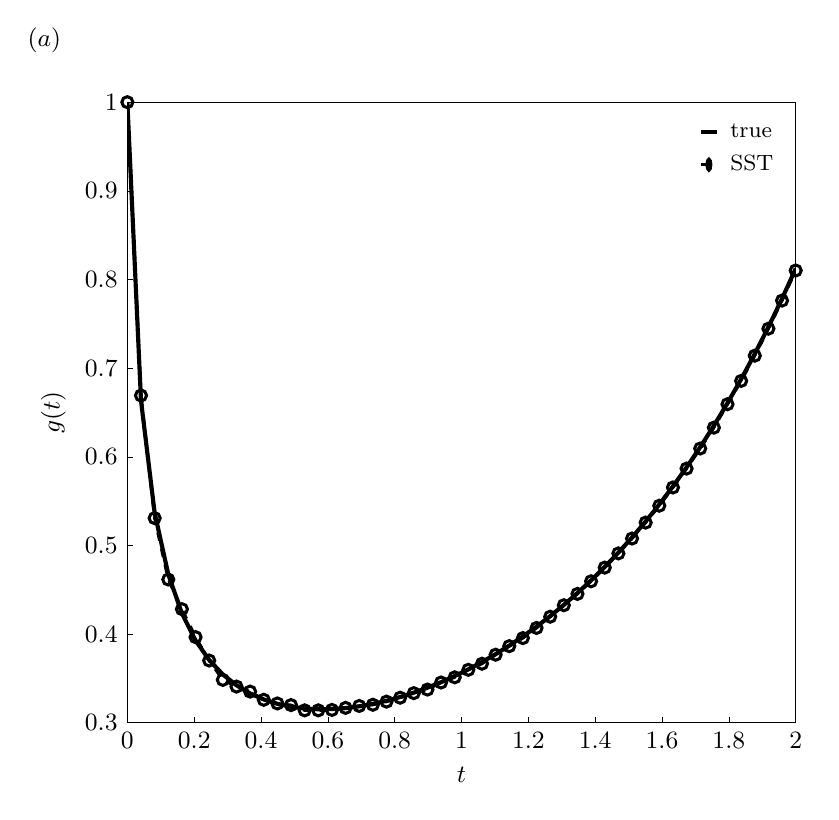
\begin{tikzpicture}

\begin{axis}[%
width=11.252in,
height=7.131in,
at={(1.887in,0.962in)},
scale only axis,
clip=true,
separate axis lines,
every outer x axis line/.append style={black},
every x tick label/.append style={font=\color{black}},
every x tick/.append style={black},
xmin=0,
xmax=2,
xlabel={$t$},
every outer y axis line/.append style={black},
every y tick label/.append style={font=\color{black}},
every y tick/.append style={black},
ymin=0.3,
ymax=1,
ylabel={$g(t)$},
axis background/.style={fill=white},
legend style={legend cell align=left, align=left},
clip=true,
clip mode=individual,
axis lines=box,
xtick pos=bottom,
ytick pos=left,
tick align=inside,
major tick length=2pt,
width=0.7\linewidth,
height=0.65\linewidth,
every axis/.append style={font=\fontsize{9}{9}\selectfont},xlabel style={font=\fontsize{9}{9}\selectfont},title style={font=\fontsize{9}{9}\selectfont},
legend style={font=\fontsize{8}{9}\selectfont,inner sep=1pt,row sep=1pt,column sep=2pt,nodes={scale=1.00},draw=none},legend image post style={xscale=0.35},
legend columns=1,
scaled x ticks=false,
tick label style={/pgf/number format/fixed,/pgf/number format/precision=2},
every x tick label/.append style={font=\fontsize{9}{9}\selectfont\color{black}},
every y tick label/.append style={font=\fontsize{9}{9}\selectfont\color{black}},
,,
colormap={sigmamap}{rgb(0.0000)=(0.0200,0.1880,0.3800); rgb(0.1000)=(0.0743,0.3456,0.5616); rgb(0.2000)=(0.1918,0.4980,0.7060); rgb(0.3000)=(0.3890,0.6708,0.8226); rgb(0.4000)=(0.7552,0.8682,0.9228); rgb(0.5000)=(0.9690,0.9689,0.9689); rgb(0.6000)=(0.9425,0.8044,0.7614); rgb(0.7000)=(0.8767,0.4910,0.4020); rgb(0.8000)=(0.7869,0.2866,0.2470); rgb(0.9000)=(0.6186,0.1239,0.1568); rgb(1.0000)=(0.4040,0.0000,0.1220)}
]
\addplot [color=black, line width=1.5pt]
  table[row sep=crcr]{%
0	1\\
0.0408163265306122	0.66330675395804\\
0.0816326530612245	0.536824941129494\\
0.122448979591837	0.467466882696835\\
0.163265306122449	0.423266896705372\\
0.204081632653061	0.392783951145584\\
0.244897959183673	0.370777690358497\\
0.285714285714286	0.354468604631329\\
0.326530612244898	0.342230432206107\\
0.36734693877551	0.333042432038574\\
0.408163265306122	0.326229415862261\\
0.448979591836735	0.321326430782801\\
0.489795918367347	0.318003124620606\\
0.530612244897959	0.316019002335715\\
0.571428571428571	0.31519570292885\\
0.612244897959184	0.315399149096094\\
0.653061224489796	0.316527675802755\\
0.693877551020408	0.318503915093072\\
0.73469387755102	0.3212691167896\\
0.775510204081633	0.324779093288403\\
0.816326530612245	0.32900127412074\\
0.857142857142857	0.333912535699938\\
0.897959183673469	0.339497583456231\\
0.938775510204082	0.345747734884182\\
0.979591836734694	0.352659998591456\\
1.02040816326531	0.360236375476831\\
1.06122448979592	0.368483329251084\\
1.10204081632653	0.377411388089313\\
1.14285714285714	0.387034849440937\\
1.18367346938776	0.3973715673234\\
1.22448979591837	0.408442806704931\\
1.26530612244898	0.420273153452165\\
1.30612244897959	0.432890471193891\\
1.3469387755102	0.446325898617112\\
1.38775510204082	0.460613882363757\\
1.42857142857143	0.475792241975417\\
1.46938775510204	0.491902264338924\\
1.51020408163265	0.508988825889449\\
1.55102040816327	0.527100541482599\\
1.59183673469388	0.546289939391666\\
1.63265306122449	0.566613662349894\\
1.6734693877551	0.588132694962395\\
1.71428571428571	0.61091261817534\\
1.75510204081633	0.635023891824554\\
1.79591836734694	0.660542166602299\\
1.83673469387755	0.687548627088745\\
1.87755102040816	0.716130367800471\\
1.91836734693878	0.746380804518932\\
1.95918367346939	0.778400123482621\\
2	0.812295771362957\\
};
\addlegendentry{true}

\addplot [color=black, dashed, line width=1.1pt, mark size=2.0pt, mark=o, mark options={solid, black}]
  table[row sep=crcr]{%
0	1\\
0.0408163265306122	0.669131978952054\\
0.0816326530612245	0.530815625761453\\
0.122448979591837	0.461572038731577\\
0.163265306122449	0.428126499381252\\
0.204081632653061	0.396595186200975\\
0.244897959183673	0.370207055435072\\
0.285714285714286	0.34837607826492\\
0.326530612244898	0.340799996480598\\
0.36734693877551	0.335145490191288\\
0.408163265306122	0.325876802705544\\
0.448979591836735	0.321768597745276\\
0.489795918367347	0.319912049594763\\
0.530612244897959	0.31398495334479\\
0.571428571428571	0.313997204515448\\
0.612244897959184	0.314478299077611\\
0.653061224489796	0.3167772597657\\
0.693877551020408	0.318928667484235\\
0.73469387755102	0.320297180575997\\
0.775510204081633	0.323813698807683\\
0.816326530612245	0.328247661412773\\
0.857142857142857	0.333389122926578\\
0.897959183673469	0.33744213721697\\
0.938775510204082	0.345392063179751\\
0.979591836734694	0.351249172134897\\
1.02040816326531	0.35971284408624\\
1.06122448979592	0.366584347482057\\
1.10204081632653	0.376741786601441\\
1.14285714285714	0.386389034390955\\
1.18367346938776	0.395513055004814\\
1.22448979591837	0.406947617761363\\
1.26530612244898	0.419615540307281\\
1.30612244897959	0.432545766317335\\
1.3469387755102	0.445343882754692\\
1.38775510204082	0.459584101510697\\
1.42857142857143	0.475003561481353\\
1.46938775510204	0.491028098241514\\
1.51020408163265	0.507798149804996\\
1.55102040816327	0.525774415952527\\
1.59183673469388	0.544826733015256\\
1.63265306122449	0.565393610281706\\
1.6734693877551	0.586699025730275\\
1.71428571428571	0.609343836169864\\
1.75510204081633	0.632867063009338\\
1.79591836734694	0.659313548617411\\
1.83673469387755	0.685568801617742\\
1.87755102040816	0.714051110686585\\
1.91836734693878	0.744499584323107\\
1.95918367346939	0.776204500056826\\
2	0.810132941789997\\
};
\addlegendentry{SST}

\node[right, align=left, inner sep=0]
at (rel axis cs:-0.15,1.1) {$(a)$};
\end{axis}
\end{tikzpicture}%
    \end{minipage}
    \hfill
    \begin{minipage}[t]{0.48\textwidth}
        \centering
        \vspace{0pt}
        % This file was created by matlab2tikz.
%
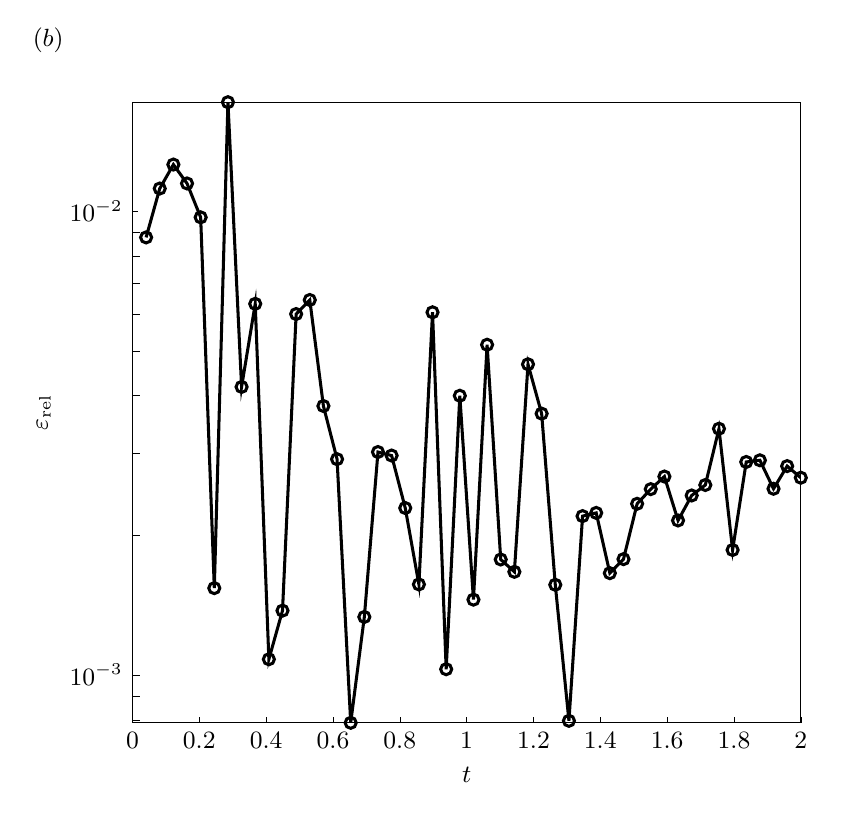
\begin{tikzpicture}

\begin{axis}[%
width=11.252in,
height=7.131in,
at={(1.887in,0.962in)},
scale only axis,
clip=true,
separate axis lines,
every outer x axis line/.append style={black},
every x tick label/.append style={font=\color{black}},
every x tick/.append style={black},
xmin=0,
xmax=2,
xlabel={$t$},
every outer y axis line/.append style={black},
every y tick label/.append style={font=\color{black}},
every y tick/.append style={black},
ymode=log,
ymin=0.000788505972857121,
ymax=0.0171877742818613,
yminorticks=true,
ylabel={$\varepsilon_{\mathrm{rel}}$},
axis background/.style={fill=white},
clip=true,
clip mode=individual,
axis lines=box,
xtick pos=bottom,
ytick pos=left,
tick align=inside,
major tick length=2pt,
width=0.7\linewidth,
height=0.65\linewidth,
every axis/.append style={font=\fontsize{9}{9}\selectfont},xlabel style={font=\fontsize{9}{9}\selectfont},title style={font=\fontsize{9}{9}\selectfont},
legend style={font=\fontsize{8}{9}\selectfont,inner sep=1pt,row sep=1pt,column sep=2pt,nodes={scale=1.00},draw=none},legend image post style={xscale=0.35},
legend columns=1,
scaled x ticks=false,
tick label style={/pgf/number format/fixed,/pgf/number format/precision=2},
every x tick label/.append style={font=\fontsize{9}{9}\selectfont\color{black}},
every y tick label/.append style={font=\fontsize{9}{9}\selectfont\color{black}},
,,
colormap={sigmamap}{rgb(0.0000)=(0.0200,0.1880,0.3800); rgb(0.1000)=(0.0743,0.3456,0.5616); rgb(0.2000)=(0.1918,0.4980,0.7060); rgb(0.3000)=(0.3890,0.6708,0.8226); rgb(0.4000)=(0.7552,0.8682,0.9228); rgb(0.5000)=(0.9690,0.9689,0.9689); rgb(0.6000)=(0.9425,0.8044,0.7614); rgb(0.7000)=(0.8767,0.4910,0.4020); rgb(0.8000)=(0.7869,0.2866,0.2470); rgb(0.9000)=(0.6186,0.1239,0.1568); rgb(1.0000)=(0.4040,0.0000,0.1220)}
]
\addplot [color=black, line width=1.1pt, mark size=2.0pt, mark=o, mark options={solid, black}, forget plot]
  table[row sep=crcr]{%
0.0408163265306122	0.00878209811562205\\
0.0816326530612245	0.0111941806492774\\
0.122448979591837	0.0126101851991099\\
0.163265306122449	0.0114811782204232\\
0.204081632653061	0.00970313334920131\\
0.244897959183673	0.00153902173259956\\
0.285714285714286	0.0171877742818613\\
0.326530612244898	0.00417974437950421\\
0.36734693877551	0.00631468530853708\\
0.408163265306122	0.00108087480641458\\
0.448979591836735	0.00137606782422971\\
0.489795918367347	0.00600284974065746\\
0.530612244897959	0.00643647684440219\\
0.571428571428571	0.00380239451954645\\
0.612244897959184	0.00291963380726255\\
0.653061224489796	0.000788505972857121\\
0.693877551020408	0.00133358609120693\\
0.73469387755102	0.00302530234874586\\
0.775510204081633	0.00297246497902733\\
0.816326530612245	0.00229060726278548\\
0.857142857142857	0.00156751459559027\\
0.897959183673469	0.00605437664190624\\
0.938775510204082	0.00102870291992012\\
0.979591836734694	0.00400052873076924\\
1.02040816326531	0.00145329962832689\\
1.06122448979592	0.00515350795621087\\
1.10204081632653	0.00177419523894462\\
1.14285714285714	0.00166862247912742\\
1.18367346938776	0.00467701383645614\\
1.22448979591837	0.00366070578064619\\
1.26530612244898	0.00156472793820272\\
1.30612244897959	0.0007962865886255\\
1.3469387755102	0.00220022155439051\\
1.38775510204082	0.00223567046606397\\
1.42857142857143	0.00165761528769134\\
1.46938775510204	0.00177711338366069\\
1.51020408163265	0.00233929710023111\\
1.55102040816327	0.00251588724675035\\
1.59183673469388	0.00267844283941867\\
1.63265306122449	0.00215323446866404\\
1.6734693877551	0.00243766286825963\\
1.71428571428571	0.0025679319084316\\
1.75510204081633	0.00339645302008812\\
1.79591836734694	0.00186001446540253\\
1.83673469387755	0.00287954246870691\\
1.87755102040816	0.00290346172621076\\
1.91836734693878	0.00252045629313518\\
1.95918367346939	0.00282068740684575\\
2	0.00266261335982454\\
};
\node[right, align=left, inner sep=0]
at (rel axis cs:-0.15,1.1) {$(b)$};
\end{axis}
\end{tikzpicture}%
    \end{minipage}
    \caption{Non-autonomous verification of the SSTE estimator. \((a)\) Normalized mean energy growth \(g(T)\) compared with the closed-form prediction. \((b)\) Relative error of the SSTE estimate as a function of final time.}
    \label{fig:nonautonomous_hutchpp}
\end{figure}
We finally validate the SSTE construction against a fully non-autonomous linear problem for which \(g(T)\) is available in closed form. The model problem is
\begin{equation}
  b(t)\frac{\partial q}{\partial t}
  =
  a(t)\frac{\partial^2 q}{\partial z^2}
  -
  c(t)\frac{\partial q}{\partial z}
  +
  r(t)q .
\end{equation}
The initial covariance is chosen as
\begin{equation}
  C_{00}^{z}(z,z')
  =
  \exp\left(
    -\frac{(z-z')^2}{\lambda^2}
  \right).
\end{equation}
For this model, the transport term only shifts the solution and does not affect the spatially integrated covariance. The normalized mean energy growth is therefore
\begin{equation}
  g(T)
  =
  \frac{\tr\left\{\mathsfbi{C}(T)\right\}}{\tr\left\{\mathsfbi{C}(0)\right\}}
  =
  \frac{
    \exp\left(2S(T)\right)
  }{
    \sqrt{1+8\tau(T)/\lambda^2}
  },
  \qquad
  \tau(T)=\int_0^T \frac{a(t)}{b(t)}\,dt,
  \qquad
  S(T)=\int_0^T \frac{r(t)}{b(t)}\,dt .
\end{equation}
This provides a direct reference for the matrix-free SSTE estimate. In the numerical test shown below, the interval is \(z\in[-64,64)\), discretized with \(N=256\) periodic grid points. The first and second spatial derivatives are approximated with eighth-order periodic finite-difference matrices, giving \(\mathsfbi{B}(t)=b(t)\mathsfbi{I}\) and \(\mathsfbi{A}(t)=a(t)\mathsfbi{D}_2-c(t)\mathsfbi{D}_1+r(t)\mathsfbi{I}\). The trace is evaluated with the uniform quadrature weight \(\Delta z\), which cancels in the normalized comparison. The final time range is \(0\le T\le 2\), with time-step target \(\Delta t=0.01\), and the initial covariance length is \(\lambda=0.5\). The scalar coefficients are
\begin{equation}
  a(t)=0.2+0.8e^{-t/5},\qquad
  c(t)=0.25+0.15\cos(1.3t),
\end{equation}
\begin{equation}
  r(t)=0.5\sqrt{t}+0.04\sin(0.9t),\qquad
  b(t)=1.0+0.2\sin(0.7t).
\end{equation}
The SSTE estimate uses \(50\) probes.

